%contents
\section*{Supplementary Methods}
\label{supplementary_methods}

\subsection*{Sea-level area changes calculations}

Sine wave (\textit{SW}) for sea-level fluctuations:


\[ SW = A sin(\omega(t) + \phi) \]    
\[ \omega = 2 \pi f \]

Surface area (\textit{A}) of a cone:

\[ A = \pi r^2 + \pi r l \]

where \textit{l} is the length of the hypotenuse of the cone, \textit{h} is the height of the cone, and \textit{r} is the radius of the cone. 

For the surface area of the upper surface of the cone we drop $\pi r^2$.

\[ A = \pi r l \]

Express the length \textit{l} in terms of \textit{r} and replace \textit{l} in the surface area equation:

\[ l = \frac{r}{cos \theta} \]

\[ A = \frac{\pi r^2}{cos \theta} \]

Calculate the radius \textit{r} of the cone by rearranging: 

\[ r = \sqrt{\frac{A cos \theta}{\pi}} \]

Calculate the height \textit{h} from the radius \textit{r} and the tangent of the angle:

\[ h = tan \theta r \]

Expressing \textit{r} and \textit{l} in terms of \textit{h} we can write area as: 

\[ A = \pi \frac{h}{tan \theta} \frac{h}{sin \theta} \]

\[ A = \pi h^2 \frac{cos \theta}{sin^2 \theta} \]

Given the current height of the cone ($h_0$) and the change in the height given a change in sea-level (\textit{h}) the new surface area of the cone is:

\[ A = \pi (h_0 - h)^2 \frac{cos \theta}{sin^2 \theta} \]

Area of the base of the cone instead to model the projection area (area as measured from an aerial view) commonly used in island biogeography. \\

Base of the cone: 

\[ A = \pi r^2 \]

Re-write with \textit{r} in terms of \textit{h}:

\[ A = \pi \left( \frac{h}{tan \theta} \right)^2 \]

Given sea-level change (\textit{h}): 

\[ A = \pi \left( \frac{h_0 - h}{tan \theta} \right) ^2 \]

Therefore, the relationship between surface area of the cone and the base of the cone is proportional and differs by a sine term.

\clearpage

\section*{Supplementary Figures}

\begin{figure}[ht]
    \centering
    \includegraphics{runtime_ed95_corr.png}
    \caption{Pearson correlation between ED\textsubscript{95} statistic and computational run time in the robustness pipeline (see Fig. \ref{fig:pipeline}, main text) for (a) $\Delta$STT, (b) $\Delta$ESTT, (c) $\Delta$NESTT, (d) number of species, (e) number of colonists for all parameter spaces. Pearson’s correlation coefficient for (a) is 0.16, (b) is 0.17, (c) is 0.12, (d) is 0.11, (e) is 0.13.}
    \label{fig:runtime_ed95_corr}
\end{figure}

\begin{figure}
    \centering
    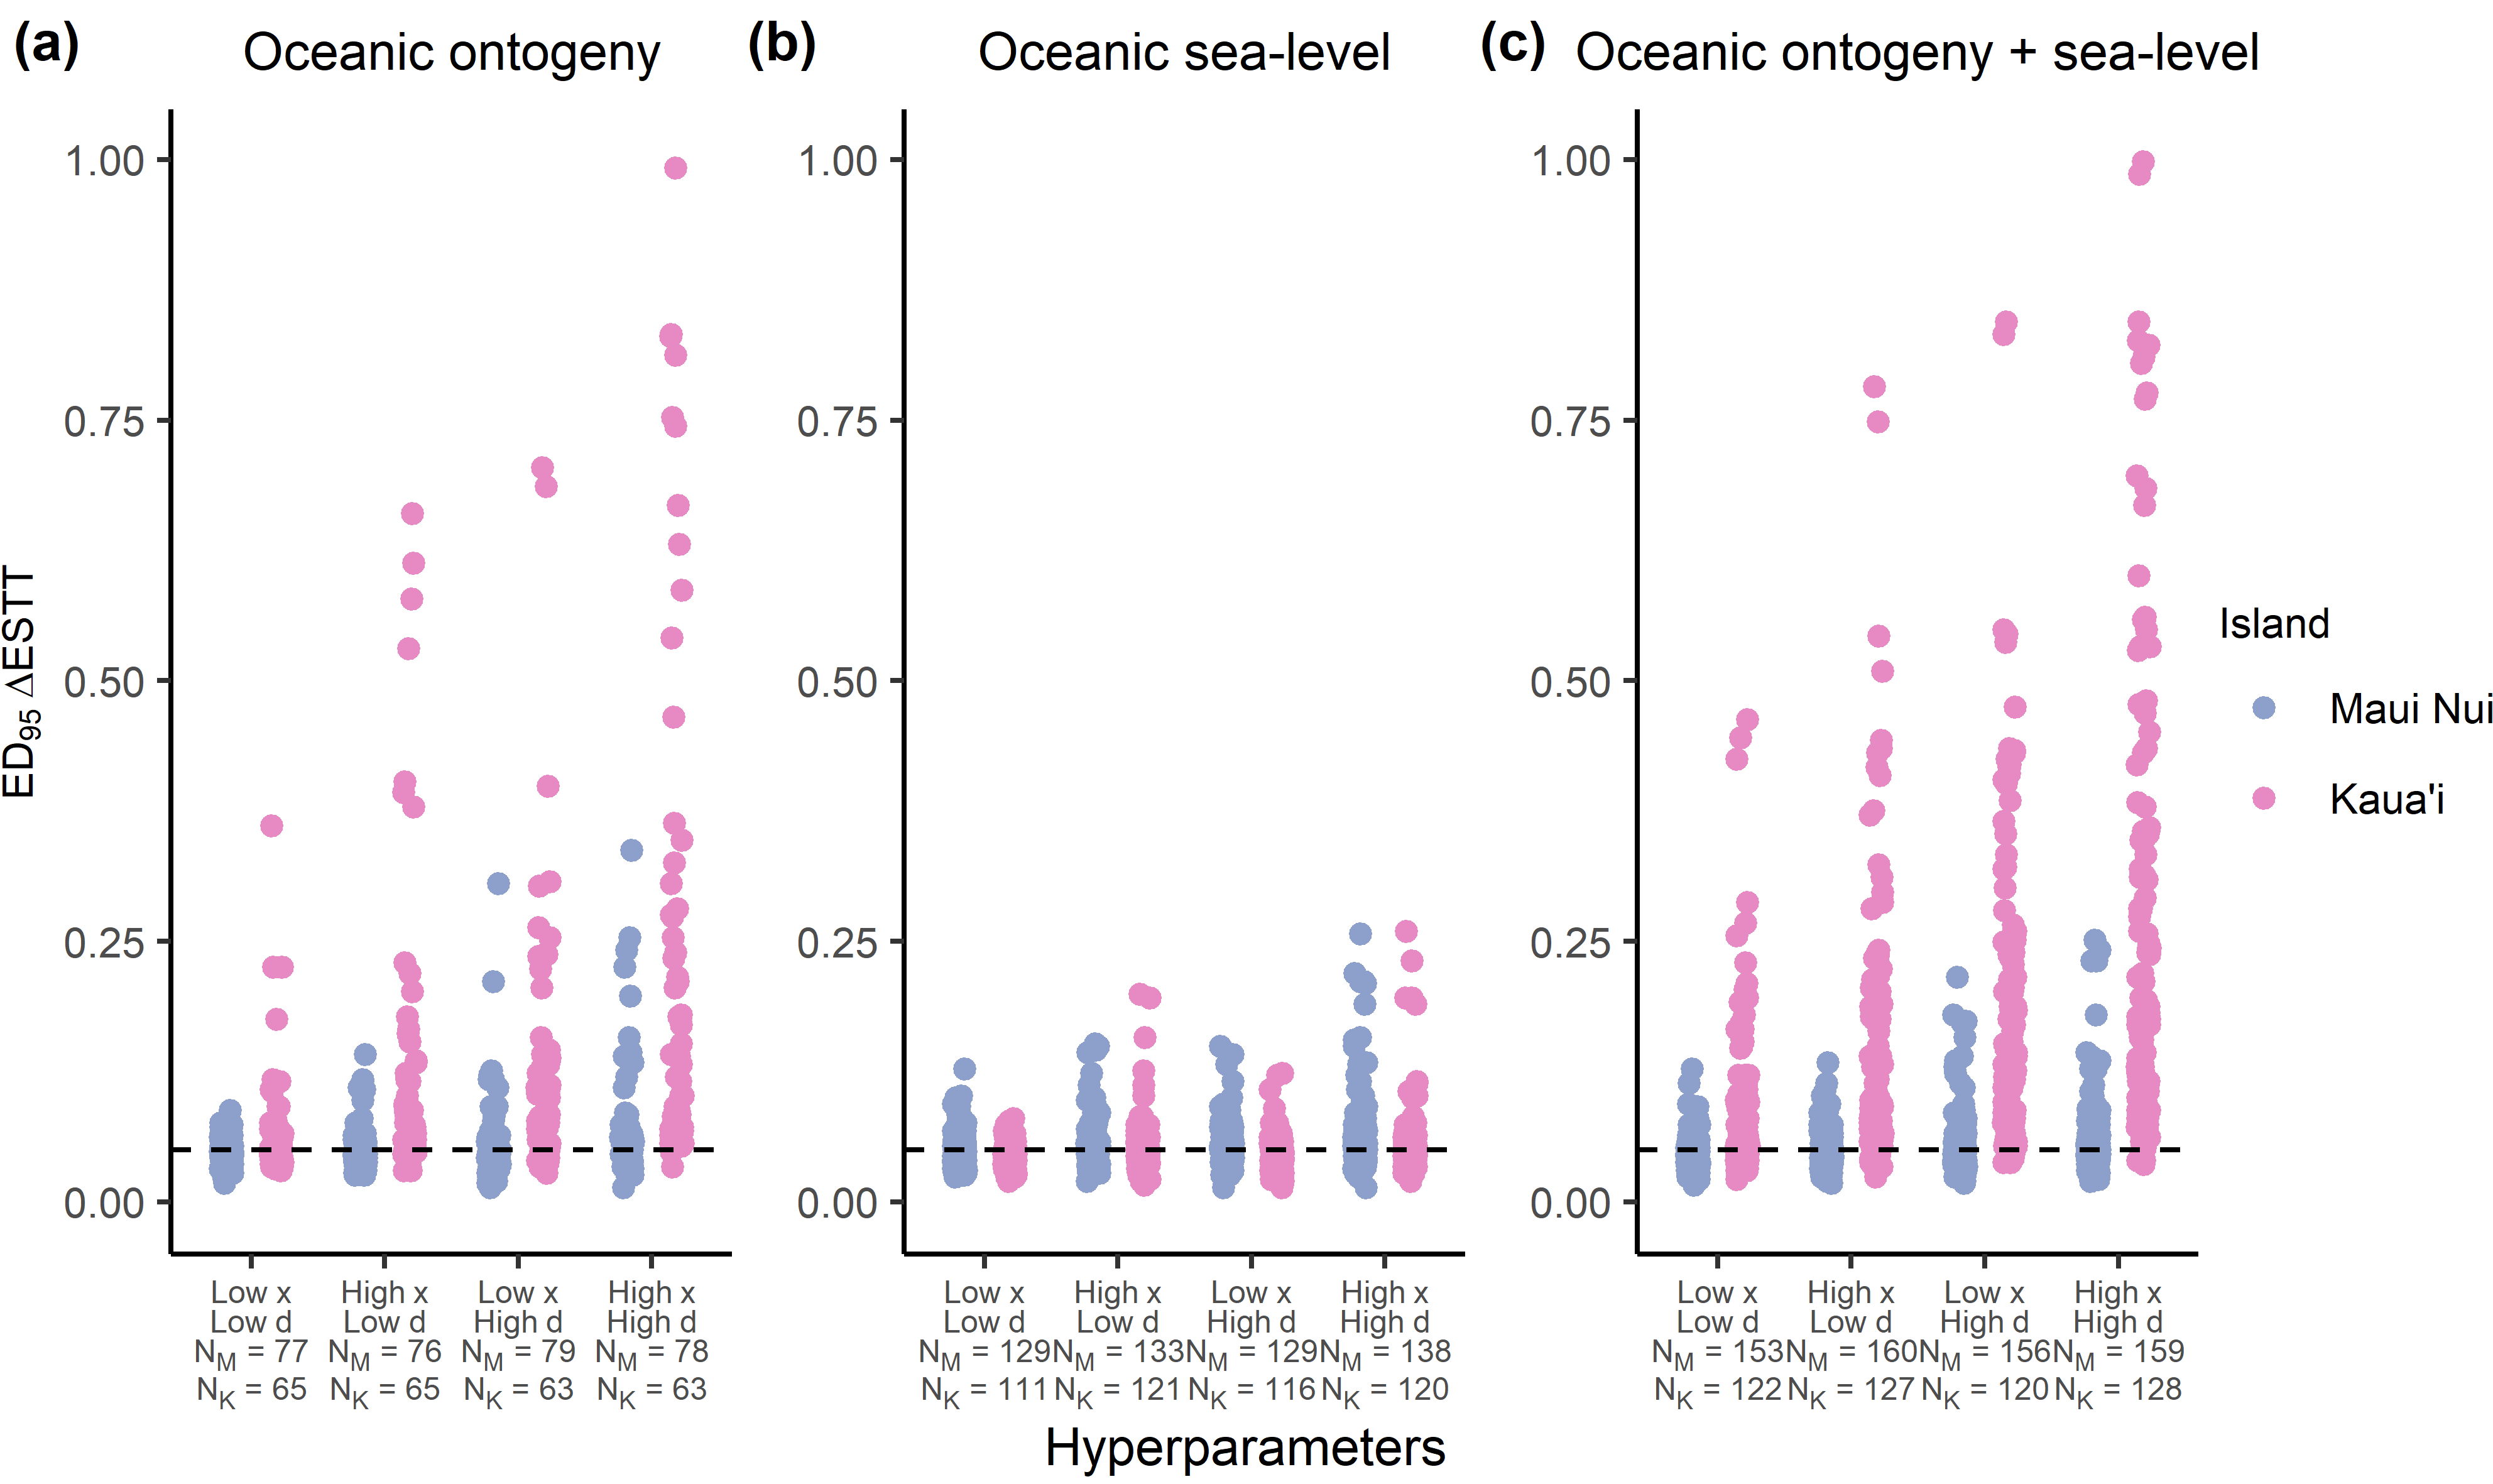
\includegraphics{Hyperparameters_endemic.png}
    \caption{Strip charts showing the distributions of the endemic ED\textsubscript{95} statistic ($\Delta$ESTT ED\textsubscript{95}) for each combination of hyperparameters (\textit{d} and \textit{x} controlling the effect of area on the rates of cladogenesis and extinction respectively). One point represents the ED\textsubscript{95} for a single parameter set with the specified hyperparameters on the \textit{x}-axis. All plots have a dashed line at 0.05 which is the null expectation of the ED\textsubscript{95}. (a) $\Delta$ESTT ED\textsubscript{95} statistic for oceanic ontogeny. (b) $\Delta$ESTT ED\textsubscript{95} statistic for oceanic sea-level. (c) $\Delta$ESTT ED\textsubscript{95} statistic for oceanic ontogeny and sea-level. Sample size for young island (green) on each strip is given in the \textit{x}-axis label by N\textsubscript{Y}. Sample size for old island (orange) on each strip is given in the \textit{x}-axis label by N\textsubscript{O}.}
    \label{fig:Hyperparameters_endemic}
\end{figure}

\begin{figure}
    \centering
    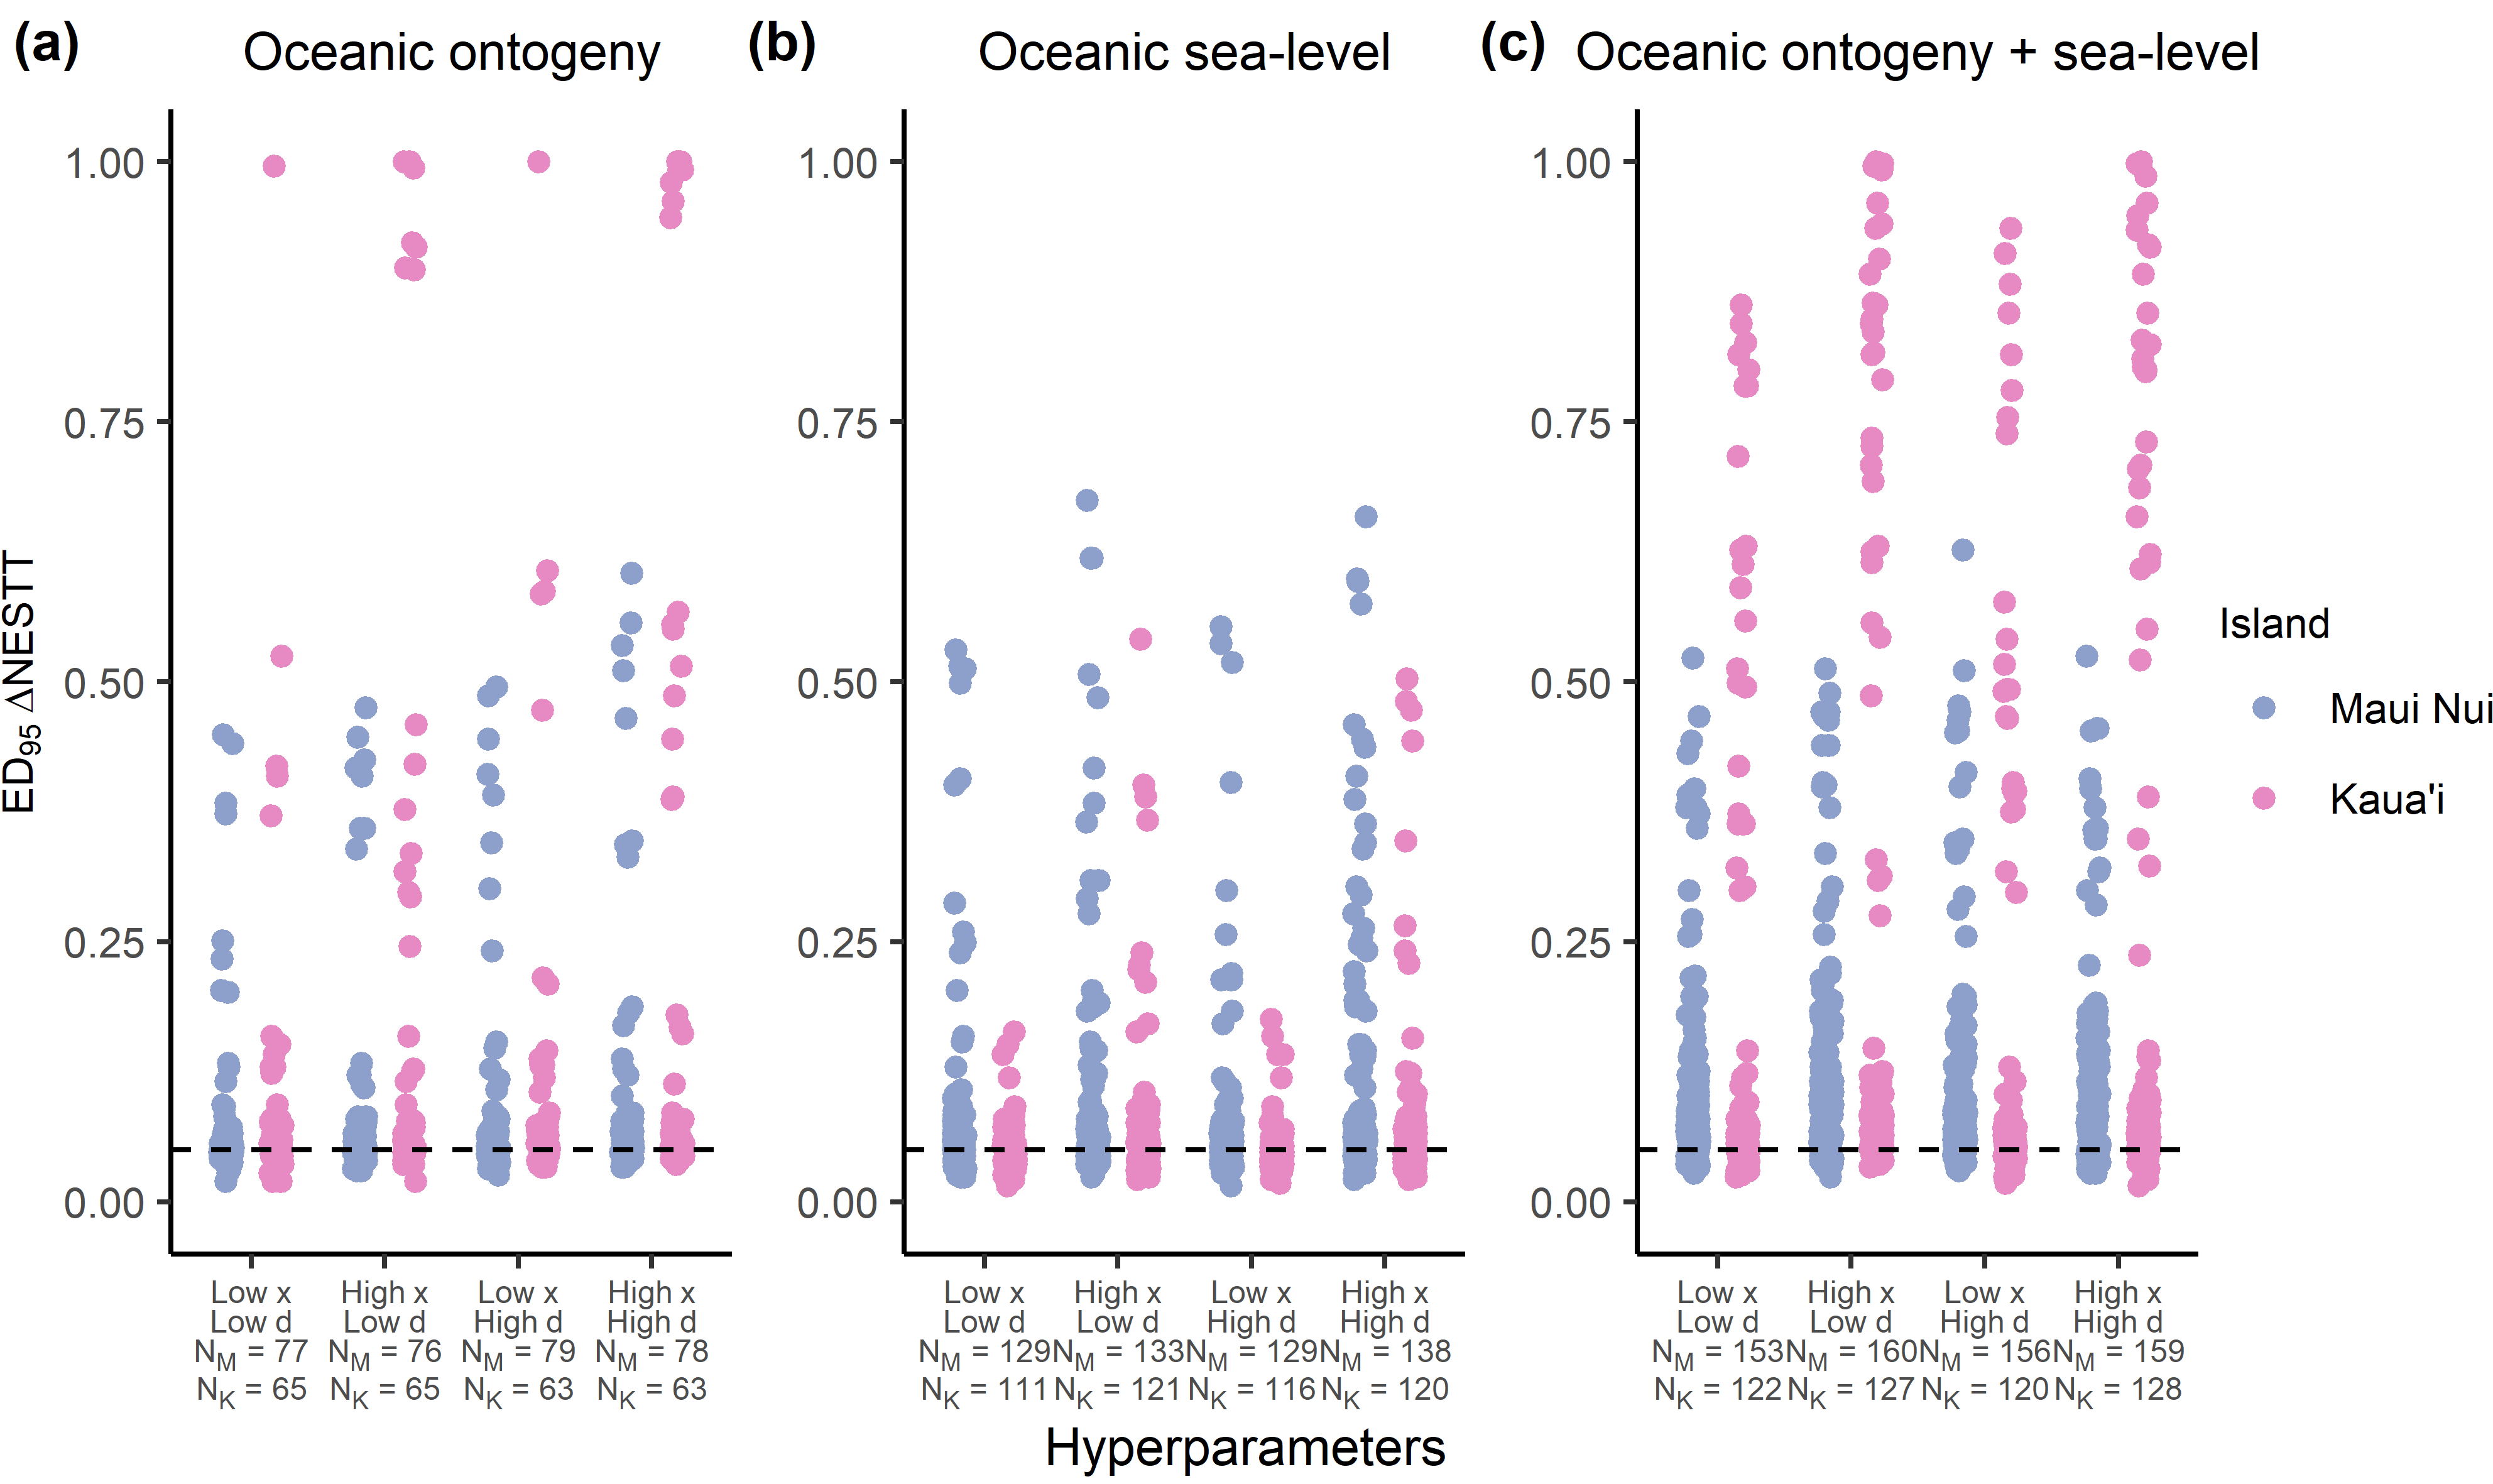
\includegraphics{Hyperparameters_nonendemic.png}
    \caption{Strip charts showing the distributions of the non-endemic ED\textsubscript{95} statistic ($\Delta$NESTT ED\textsubscript{95}) for each combination of hyperparameters (\textit{d} and \textit{x} controlling the effect of area on the rates of cladogenesis and extinction respectively). One point represents the ED\textsubscript{95} for a single parameter set with the specified hyperparameters on the \textit{x}-axis. All plots have a dashed line at 0.05 which is the null expectation of the ED\textsubscript{95}. (a) $\Delta$NESTT ED\textsubscript{95} statistic for oceanic ontogeny. (b) $\Delta$NESTT ED\textsubscript{95} statistic for oceanic sea-level. (c) $\Delta$NESTT ED\textsubscript{95} statistic for oceanic ontogeny and sea-level. Sample size for young island (green) on each strip is given in the \textit{x}-axis label by N\textsubscript{Y}. Sample size for old island (orange) on each strip is given in the \textit{x}-axis label by N\textsubscript{O}.}
    \label{fig:Hyperparameters_nonendemic}
\end{figure}
 
\begin{figure}
    \centering
    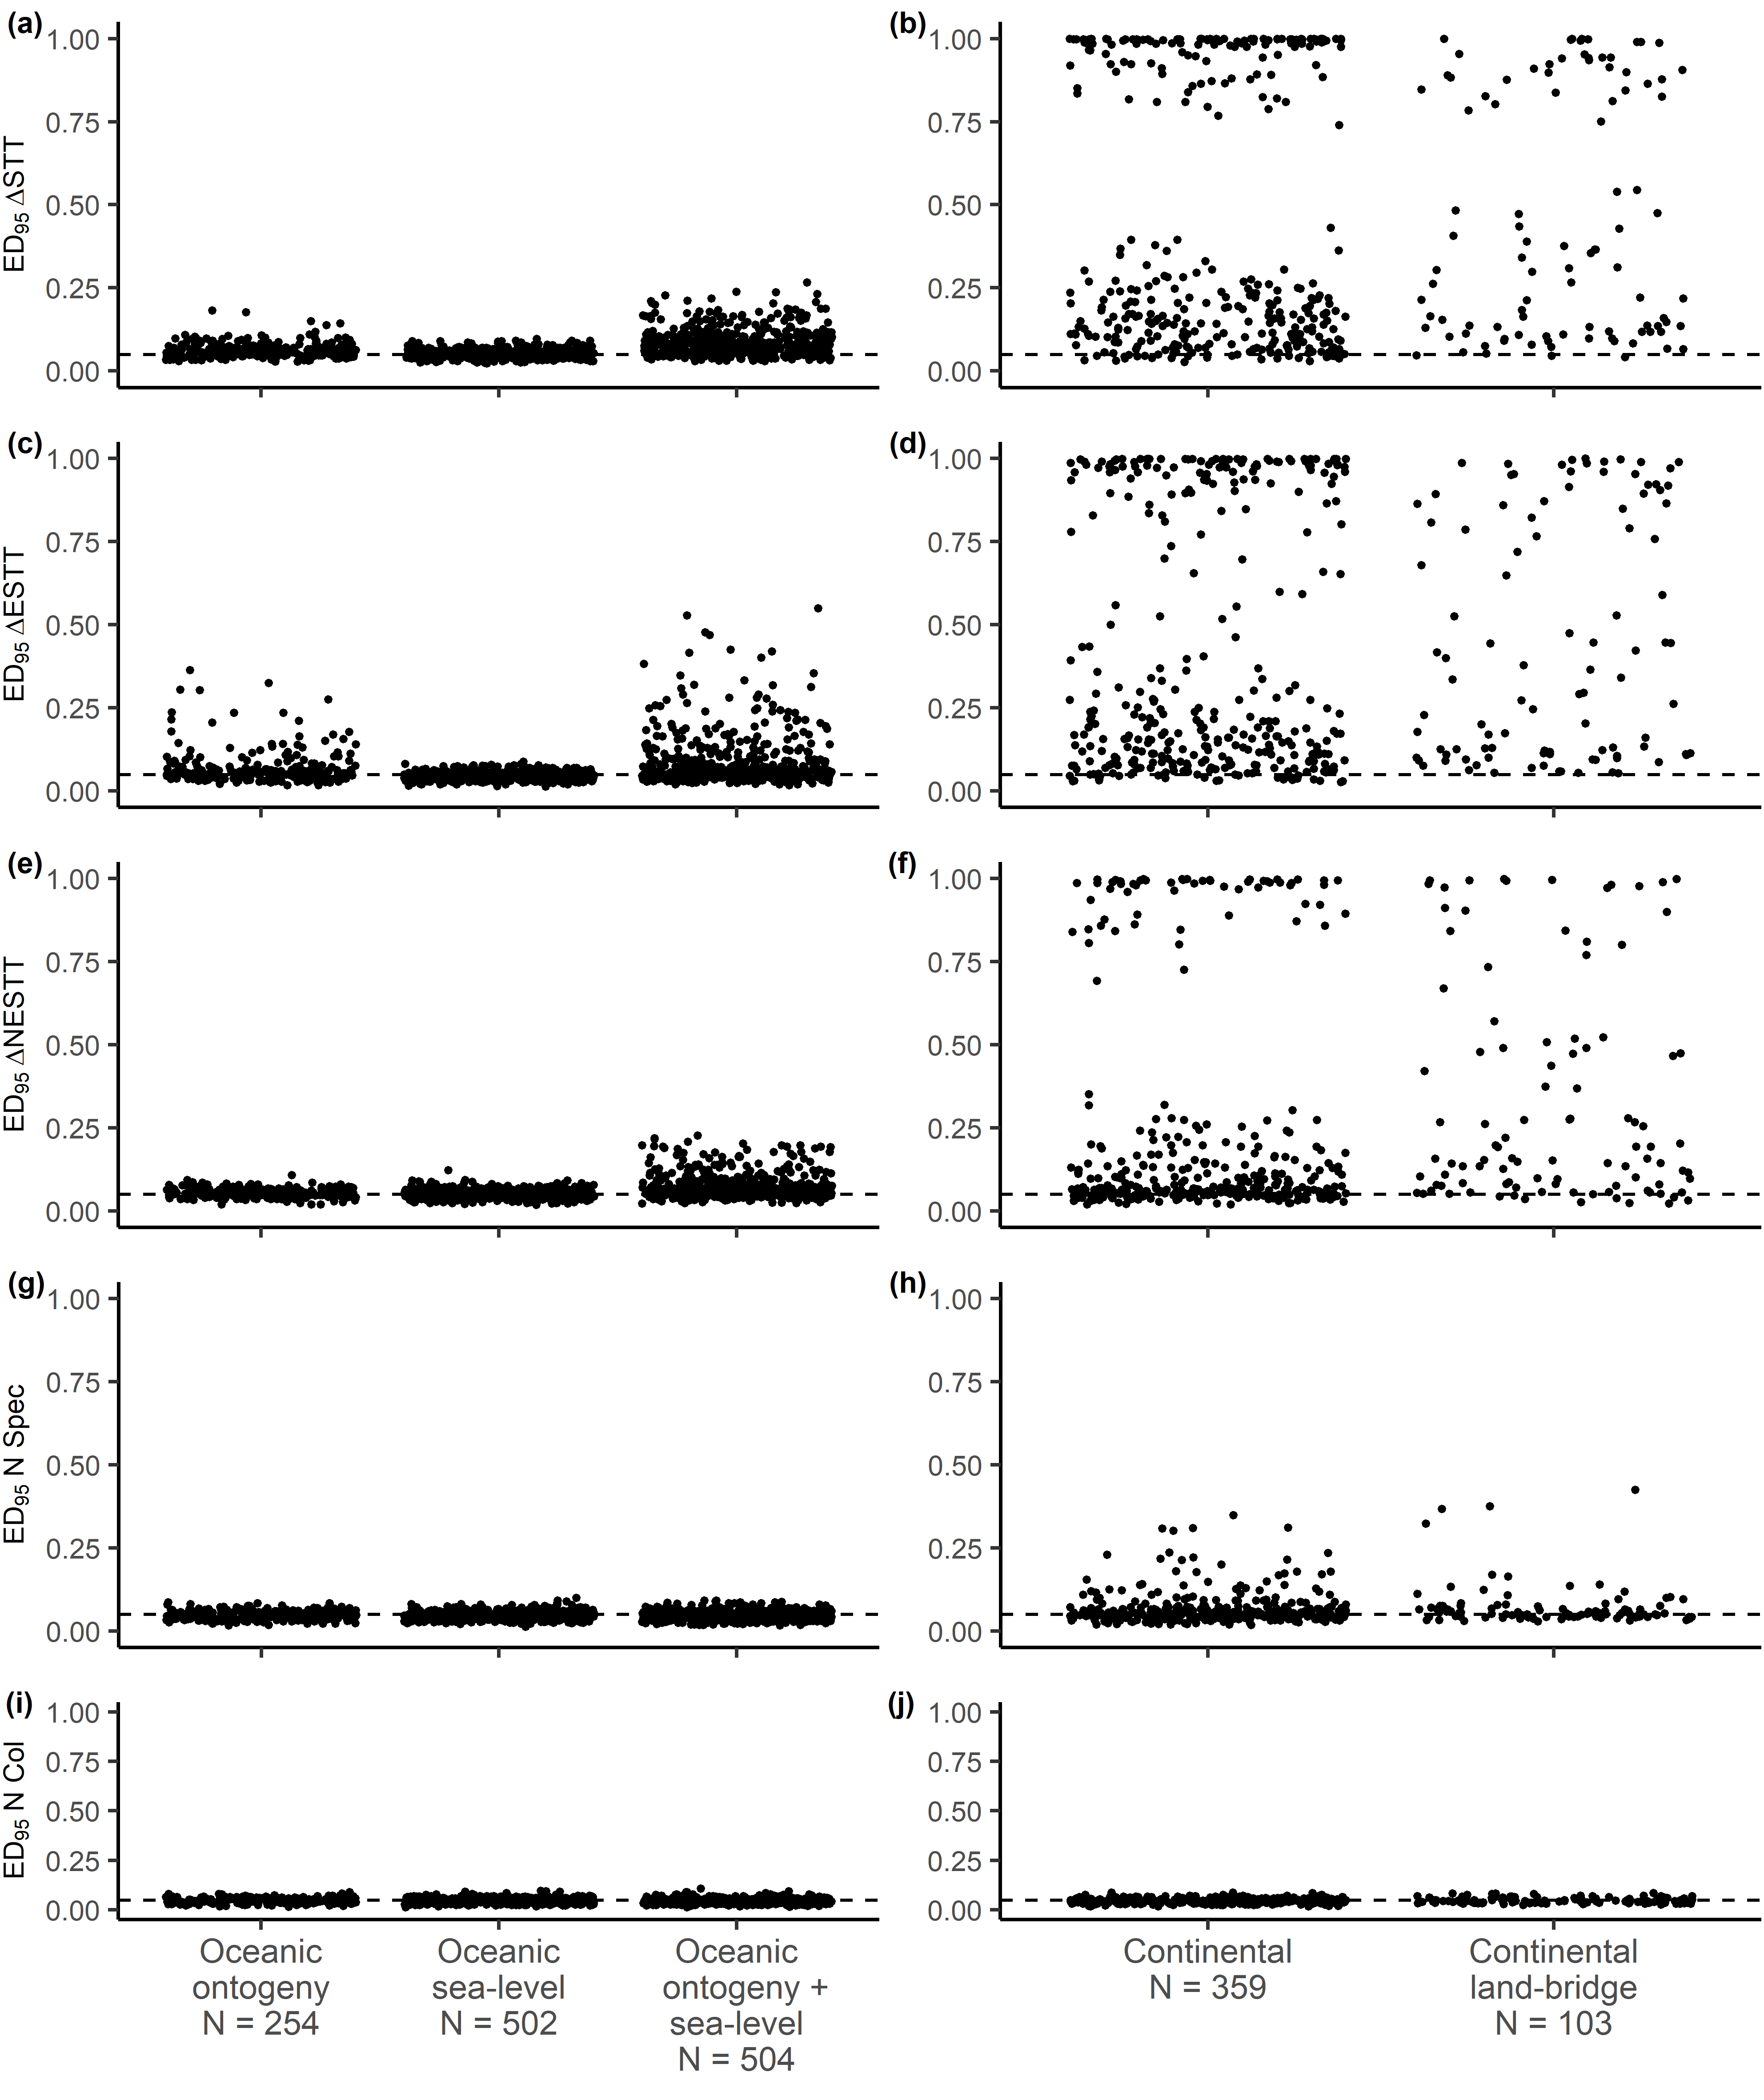
\includegraphics[width=\textwidth]{facet_scenario_cs.png}
    \caption{Strip charts showing the distribution of the ED\textsubscript{95} statistics calculated for the $\Delta$STT (a-b), $\Delta$ESTT (c-d), $\Delta$NESTT (e-f), number of species at the present (N Spec) (g-h), and number of colonists at the present (N Col) (i-j) for each geodynamic scenario. The scenarios are: oceanic ontogeny, oceanic sea-level, and oceanic ontogeny sea-level (green), as well as two continental scenarios: continental island and continental land-bridge (orange). Each point represents the ED\textsubscript{95} for a single parameter setting. Dashed line at 0.05 is the null expectation of the ED\textsubscript{95} error. N shows the sample size for each strip on the \textit{x}-axis.}
    \label{fig:facet_scenario_cs}
\end{figure}

\begin{figure}
    \centering
    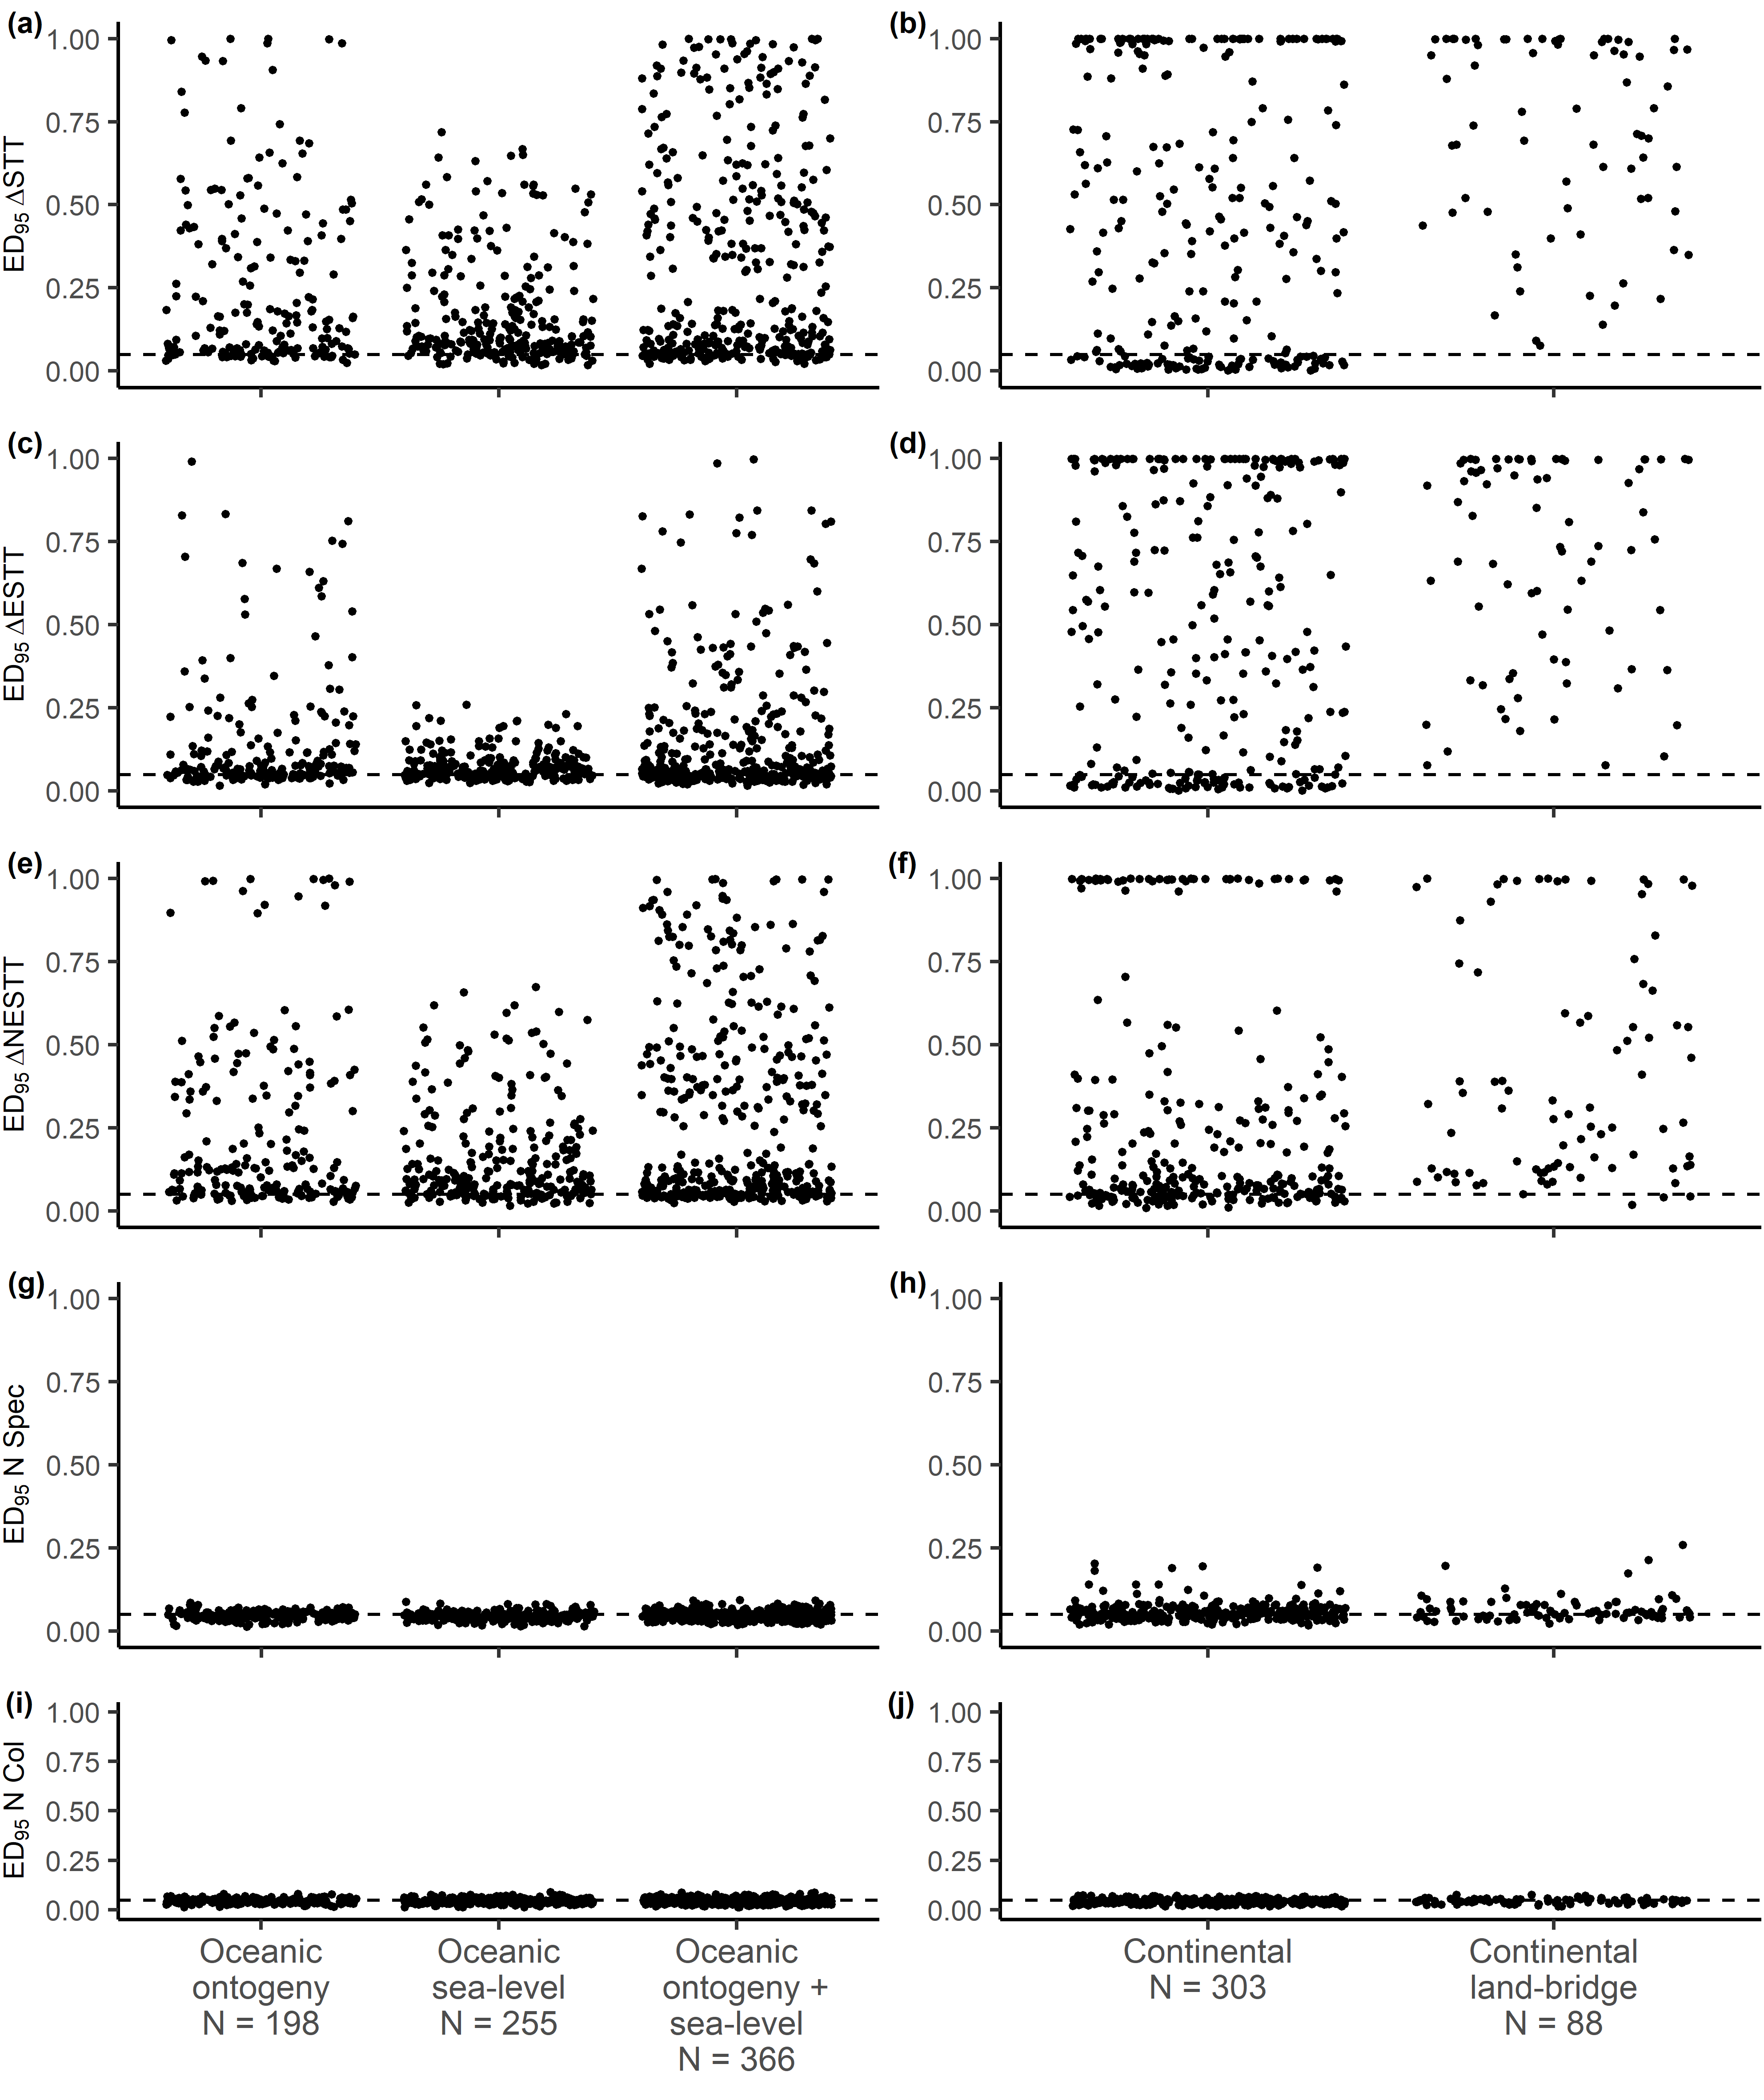
\includegraphics[width=\textwidth]{facet_scenario_iw.png}
    \caption{Strip charts showing the distribution of the ED\textsubscript{95} statistics calculated for the $\Delta$STT (a-b), $\Delta$ESTT (c-d), $\Delta$NESTT (e-f), number of species at the present (N Spec) (g-h), and number of colonists at the present (N Col) (i-j) for each geodynamic scenario. The scenarios are: oceanic ontogeny, oceanic sea-level, and oceanic ontogeny sea-level (green), as well as two continental scenarios: continental island and continental land-bridge (orange). Each point represents the ED\textsubscript{95} for a single parameter setting. Dashed line at 0.05 is the null expectation of the ED\textsubscript{95} error. N shows the sample size for each strip on the \textit{x}-axis.}
    \label{fig:facet_scenario_iw}
\end{figure}
\begin{figure}
    \centering
    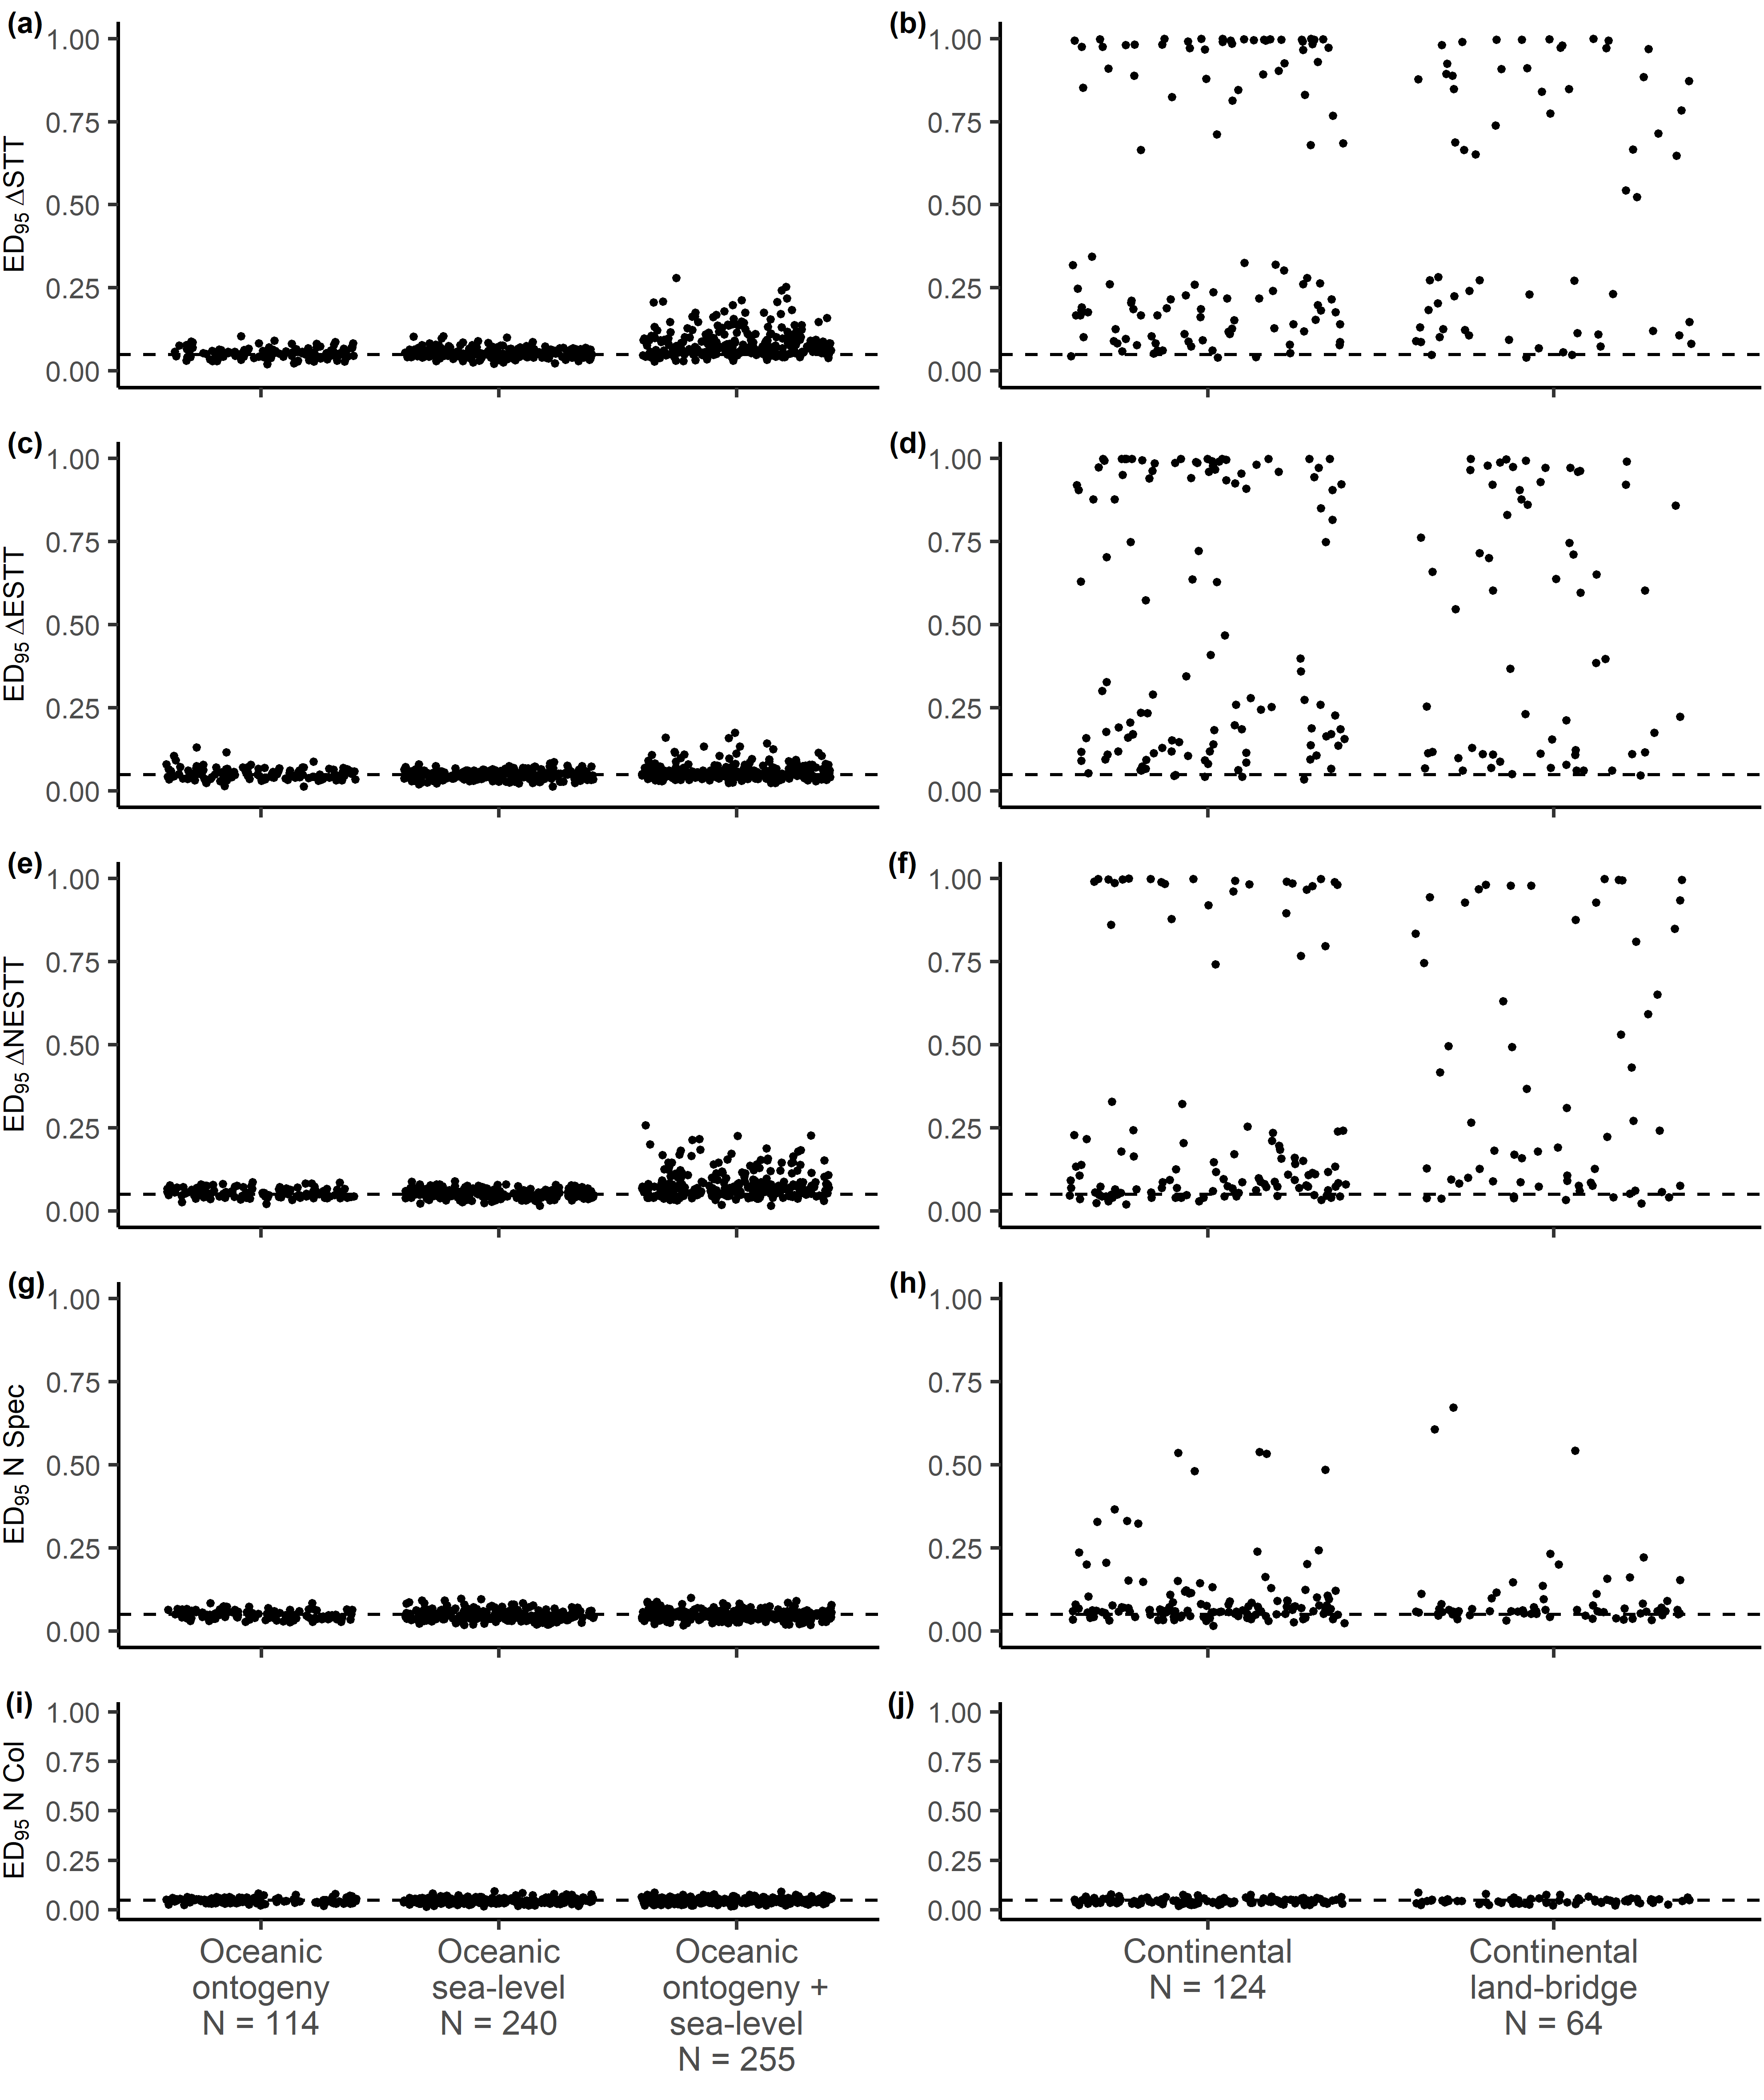
\includegraphics[width=\textwidth]{facet_scenario_di.png}
    \caption{Strip charts showing the distribution of the ED\textsubscript{95} statistics calculated for the $\Delta$STT (a-b), $\Delta$ESTT (c-d), $\Delta$NESTT (e-f), number of species at the present (N Spec) (g-h), and number of colonists at the present (N Col) (i-j) for each geodynamic scenario. The scenarios are: oceanic ontogeny, oceanic sea-level, and oceanic ontogeny sea-level (green), as well as two continental scenarios: continental island and continental land-bridge (orange). Each point represents the ED\textsubscript{95} for a single parameter setting. Dashed line at 0.05 is the null expectation of the ED\textsubscript{95} error. N shows the sample size for each strip on the \textit{x}-axis.}
    \label{fig:facet_scenario_di}
\end{figure}

\begin{figure}
    \centering
    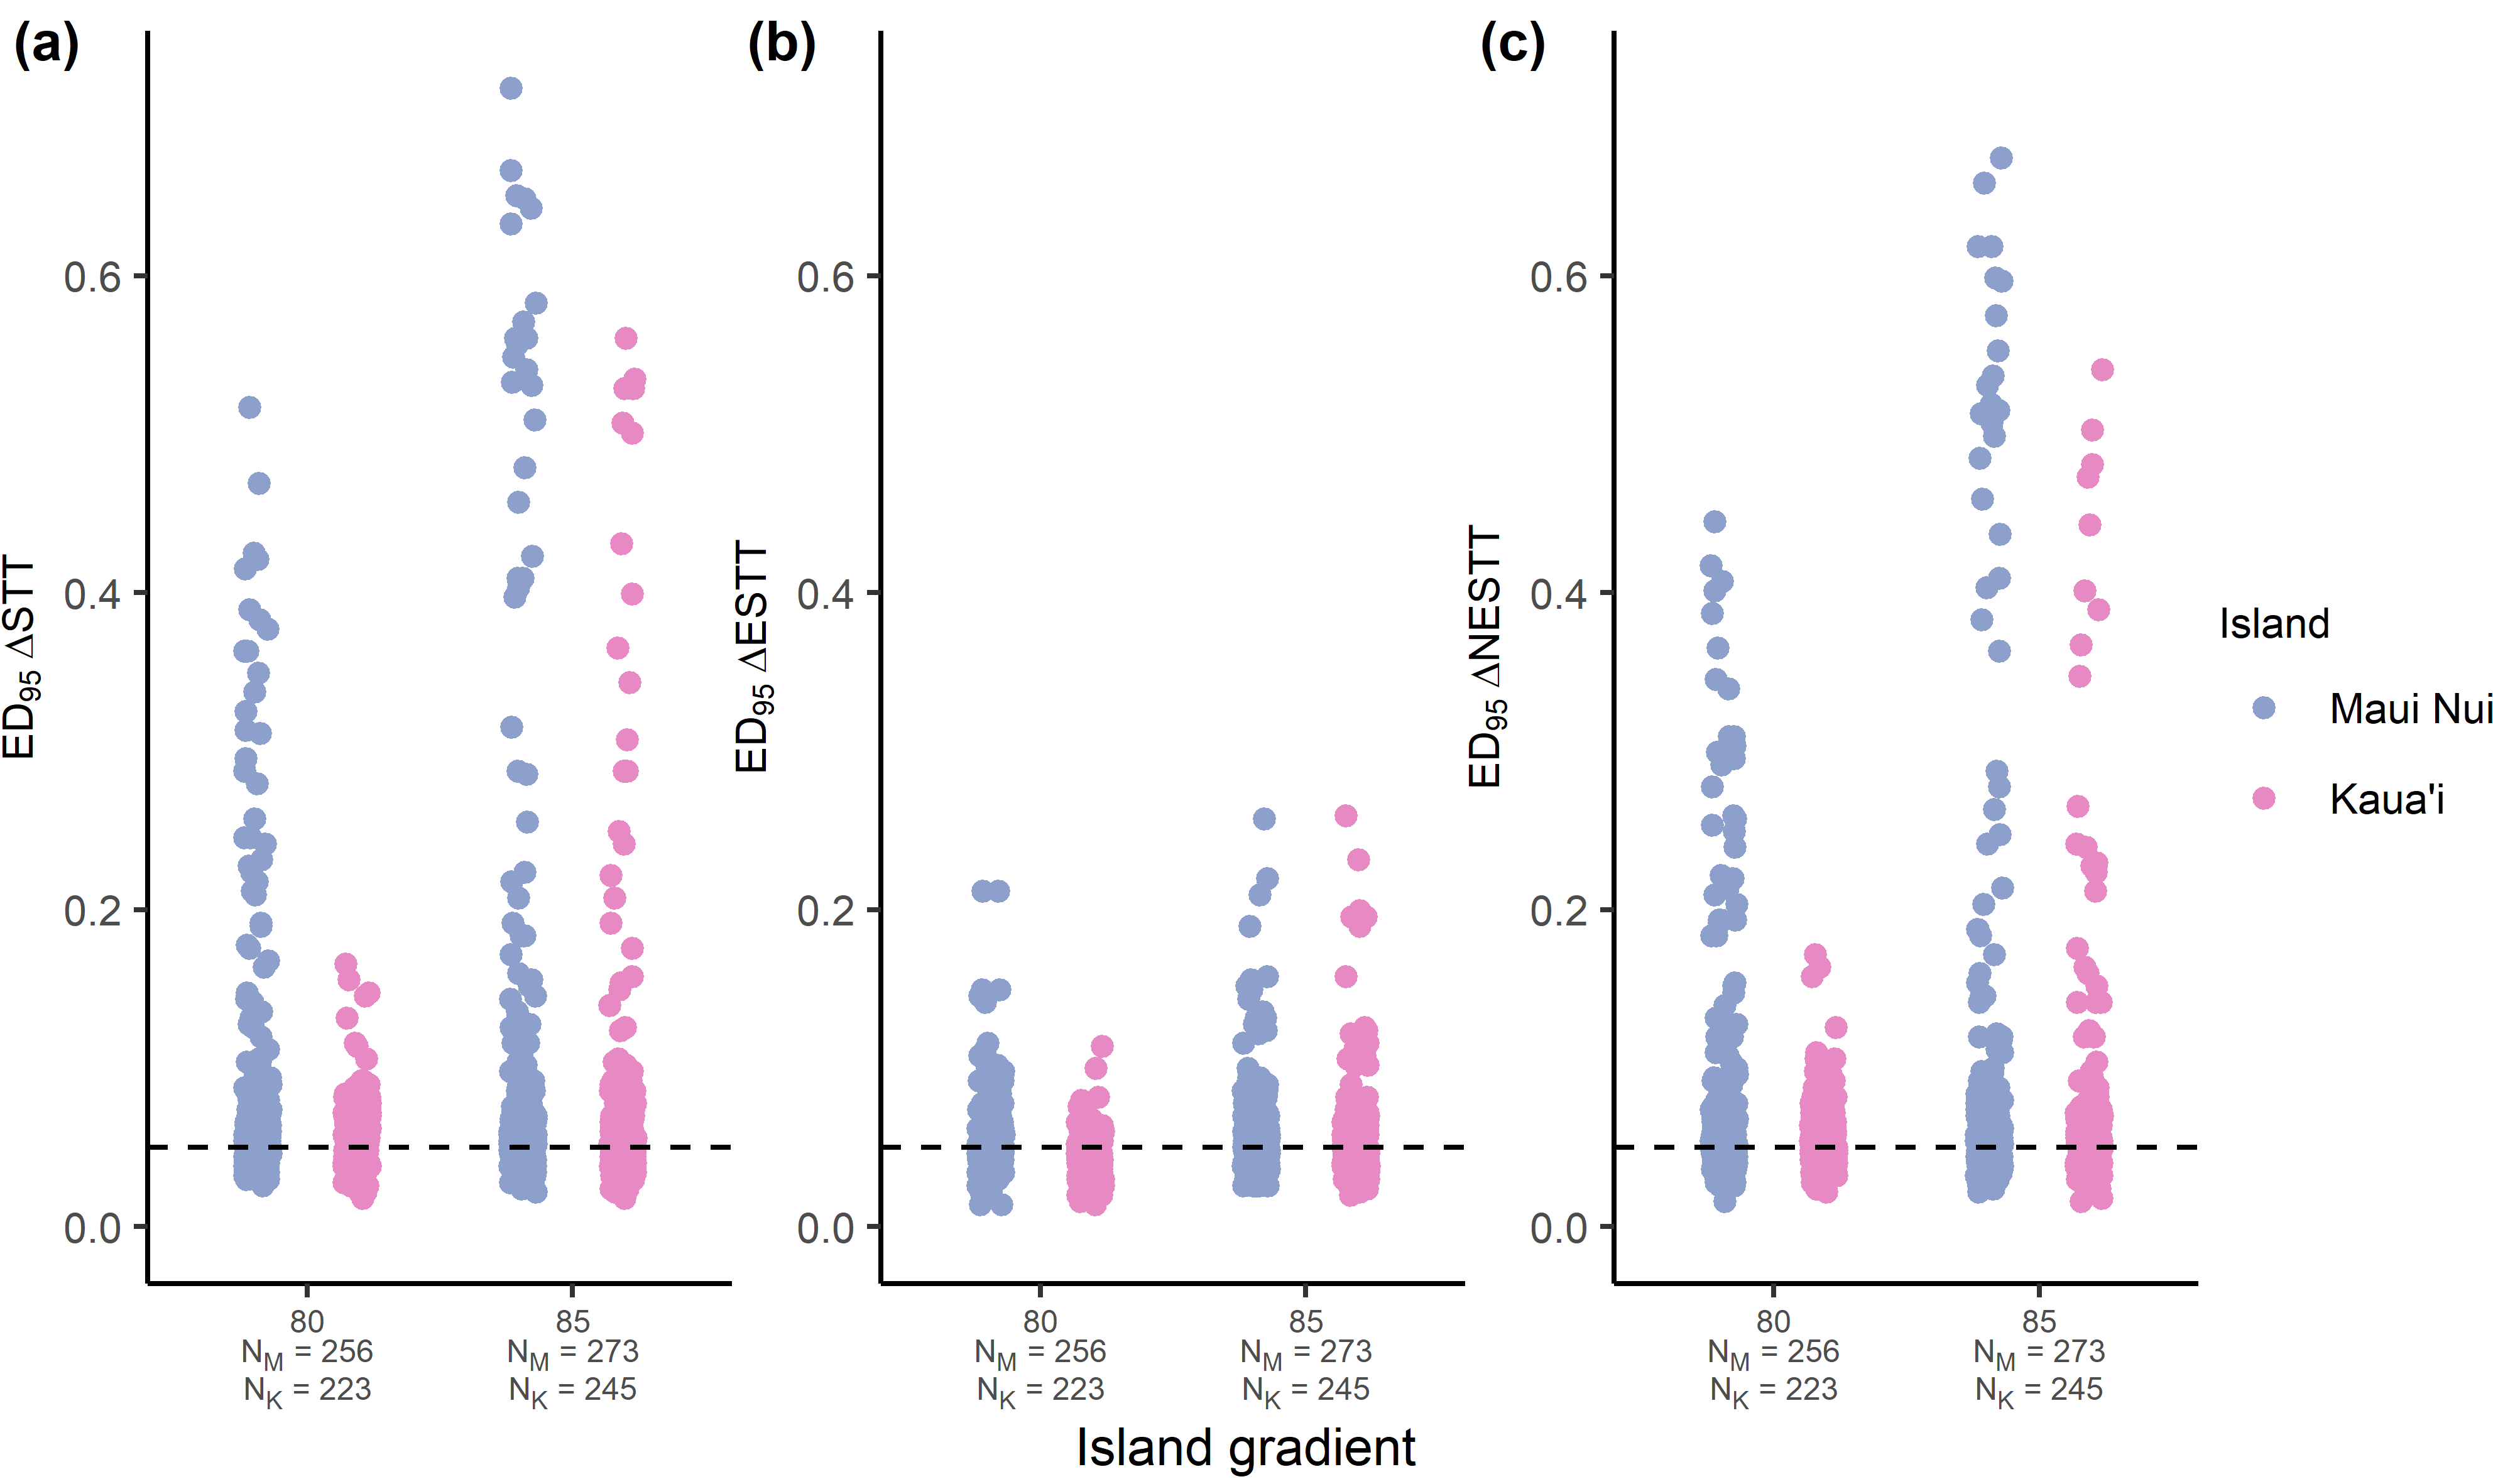
\includegraphics{oceanic_sea_level_gradient_nltt.png}
    \caption{Strip charts showing the distributions of the ED\textsubscript{95} statistic for each combination of island gradients for oceanic sea-level (without ontogeny). One point represents the ED\textsubscript{95} for a single parameter set with the specified island gradient on the \textit{x}-axis. All plots have a dashed line at 0.05 which is the null expectation of the ED\textsubscript{95}. (a) $\Delta$STT ED\textsubscript{95} statistic, (b) $\Delta$ESTT ED\textsubscript{95} statistic, (c) $\Delta$NESTT ED\textsubscript{95} statistic for oceanic sea-level. Sample size for young island (green) on each strip is given in the \textit{x}-axis label by N\textsubscript{Y}. Sample size for old island (orange) on each strip is given in the \textit{x}-axis label by N\textsubscript{O}.}
    \label{fig:oceanic_sea_level_gradient_nltt}
\end{figure}

\begin{figure}
    \centering
    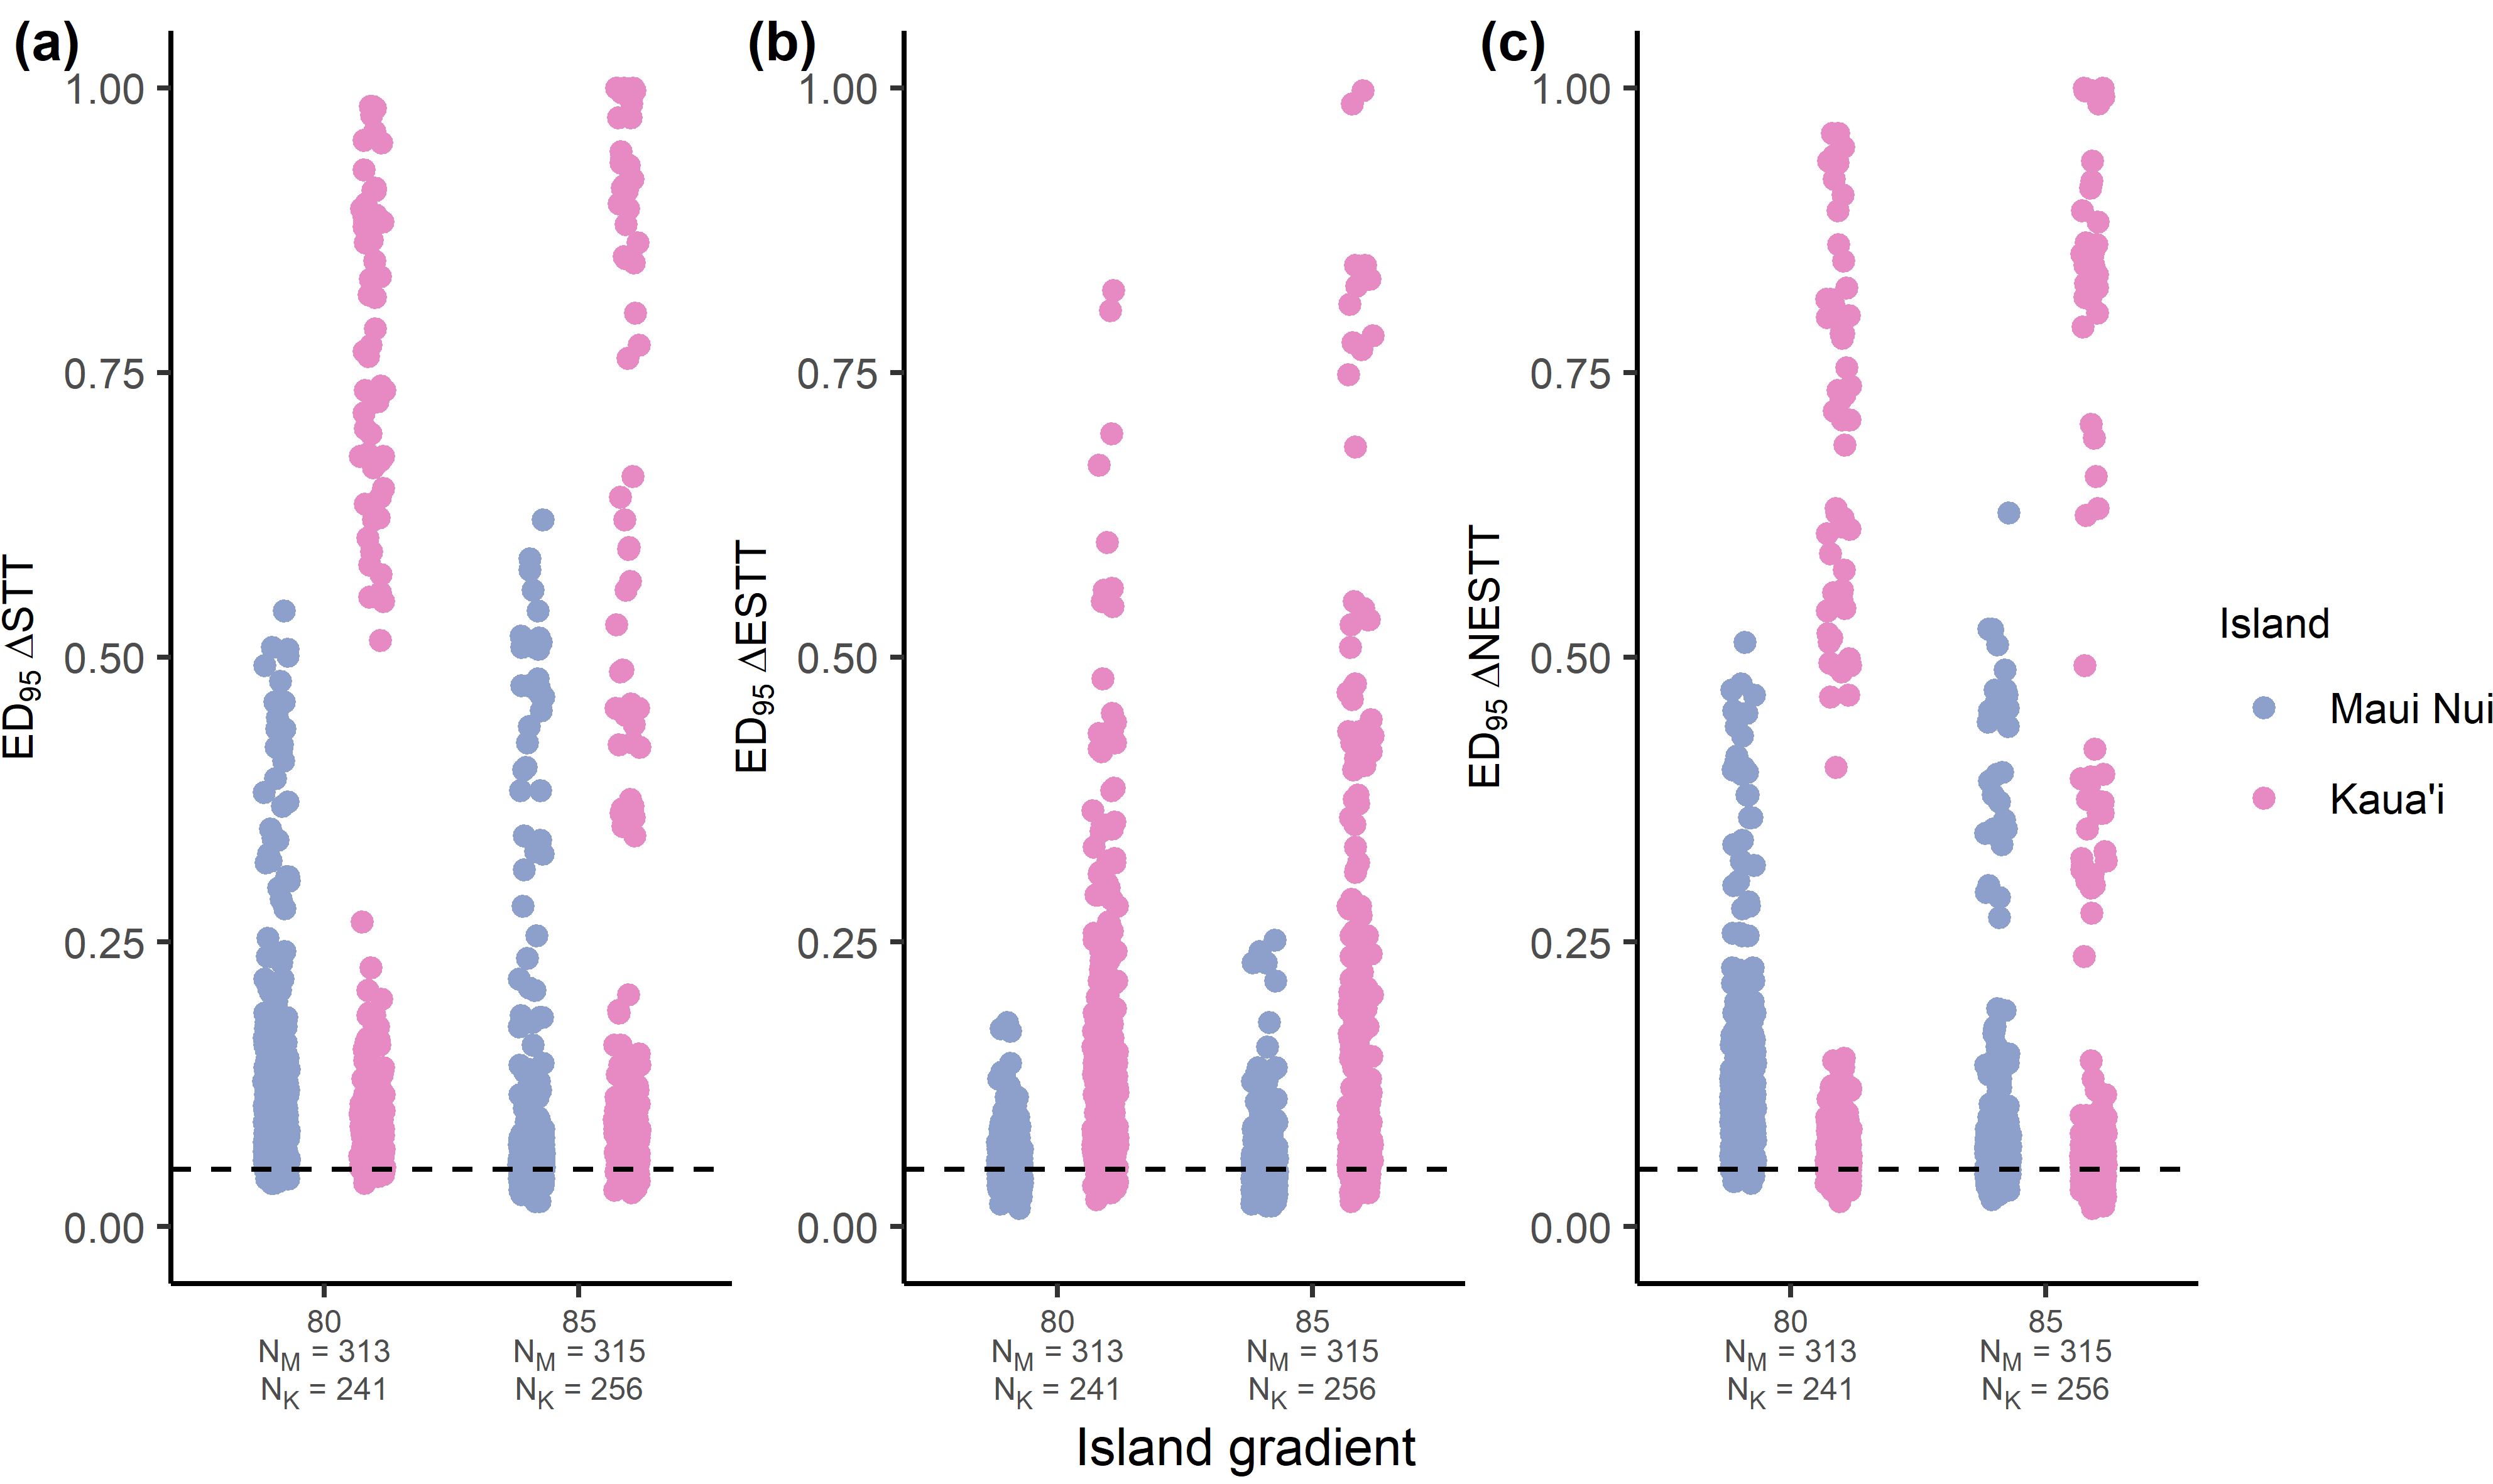
\includegraphics{oceanic_ontogeny_sea_level_gradient_nltt.png}
    \caption{Strip charts showing the distributions of the ED\textsubscript{95} statistic for each combination of island gradients for oceanic ontogeny sea-level. One point represents the ED\textsubscript{95} for a single parameter set with the specified island gradient on the \textit{x}-axis. All plots have a dashed line at 0.05 which is the null expectation of the ED\textsubscript{95}. (a) $\Delta$STT ED\textsubscript{95} statistic, (b) $\Delta$ESTT ED\textsubscript{95} statistic, (c) $\Delta$NESTT ED\textsubscript{95} statistic for oceanic ontogeny sea-level. Sample size for young island (green) on each strip is given in the \textit{x}-axis label by N\textsubscript{Y}. Sample size for old island (orange) on each strip is given in the \textit{x}-axis label by N\textsubscript{O}.}
    \label{fig:oceanic_ontogeny_sea_level_gradient_nltt}
\end{figure}

\begin{figure}
    \centering
    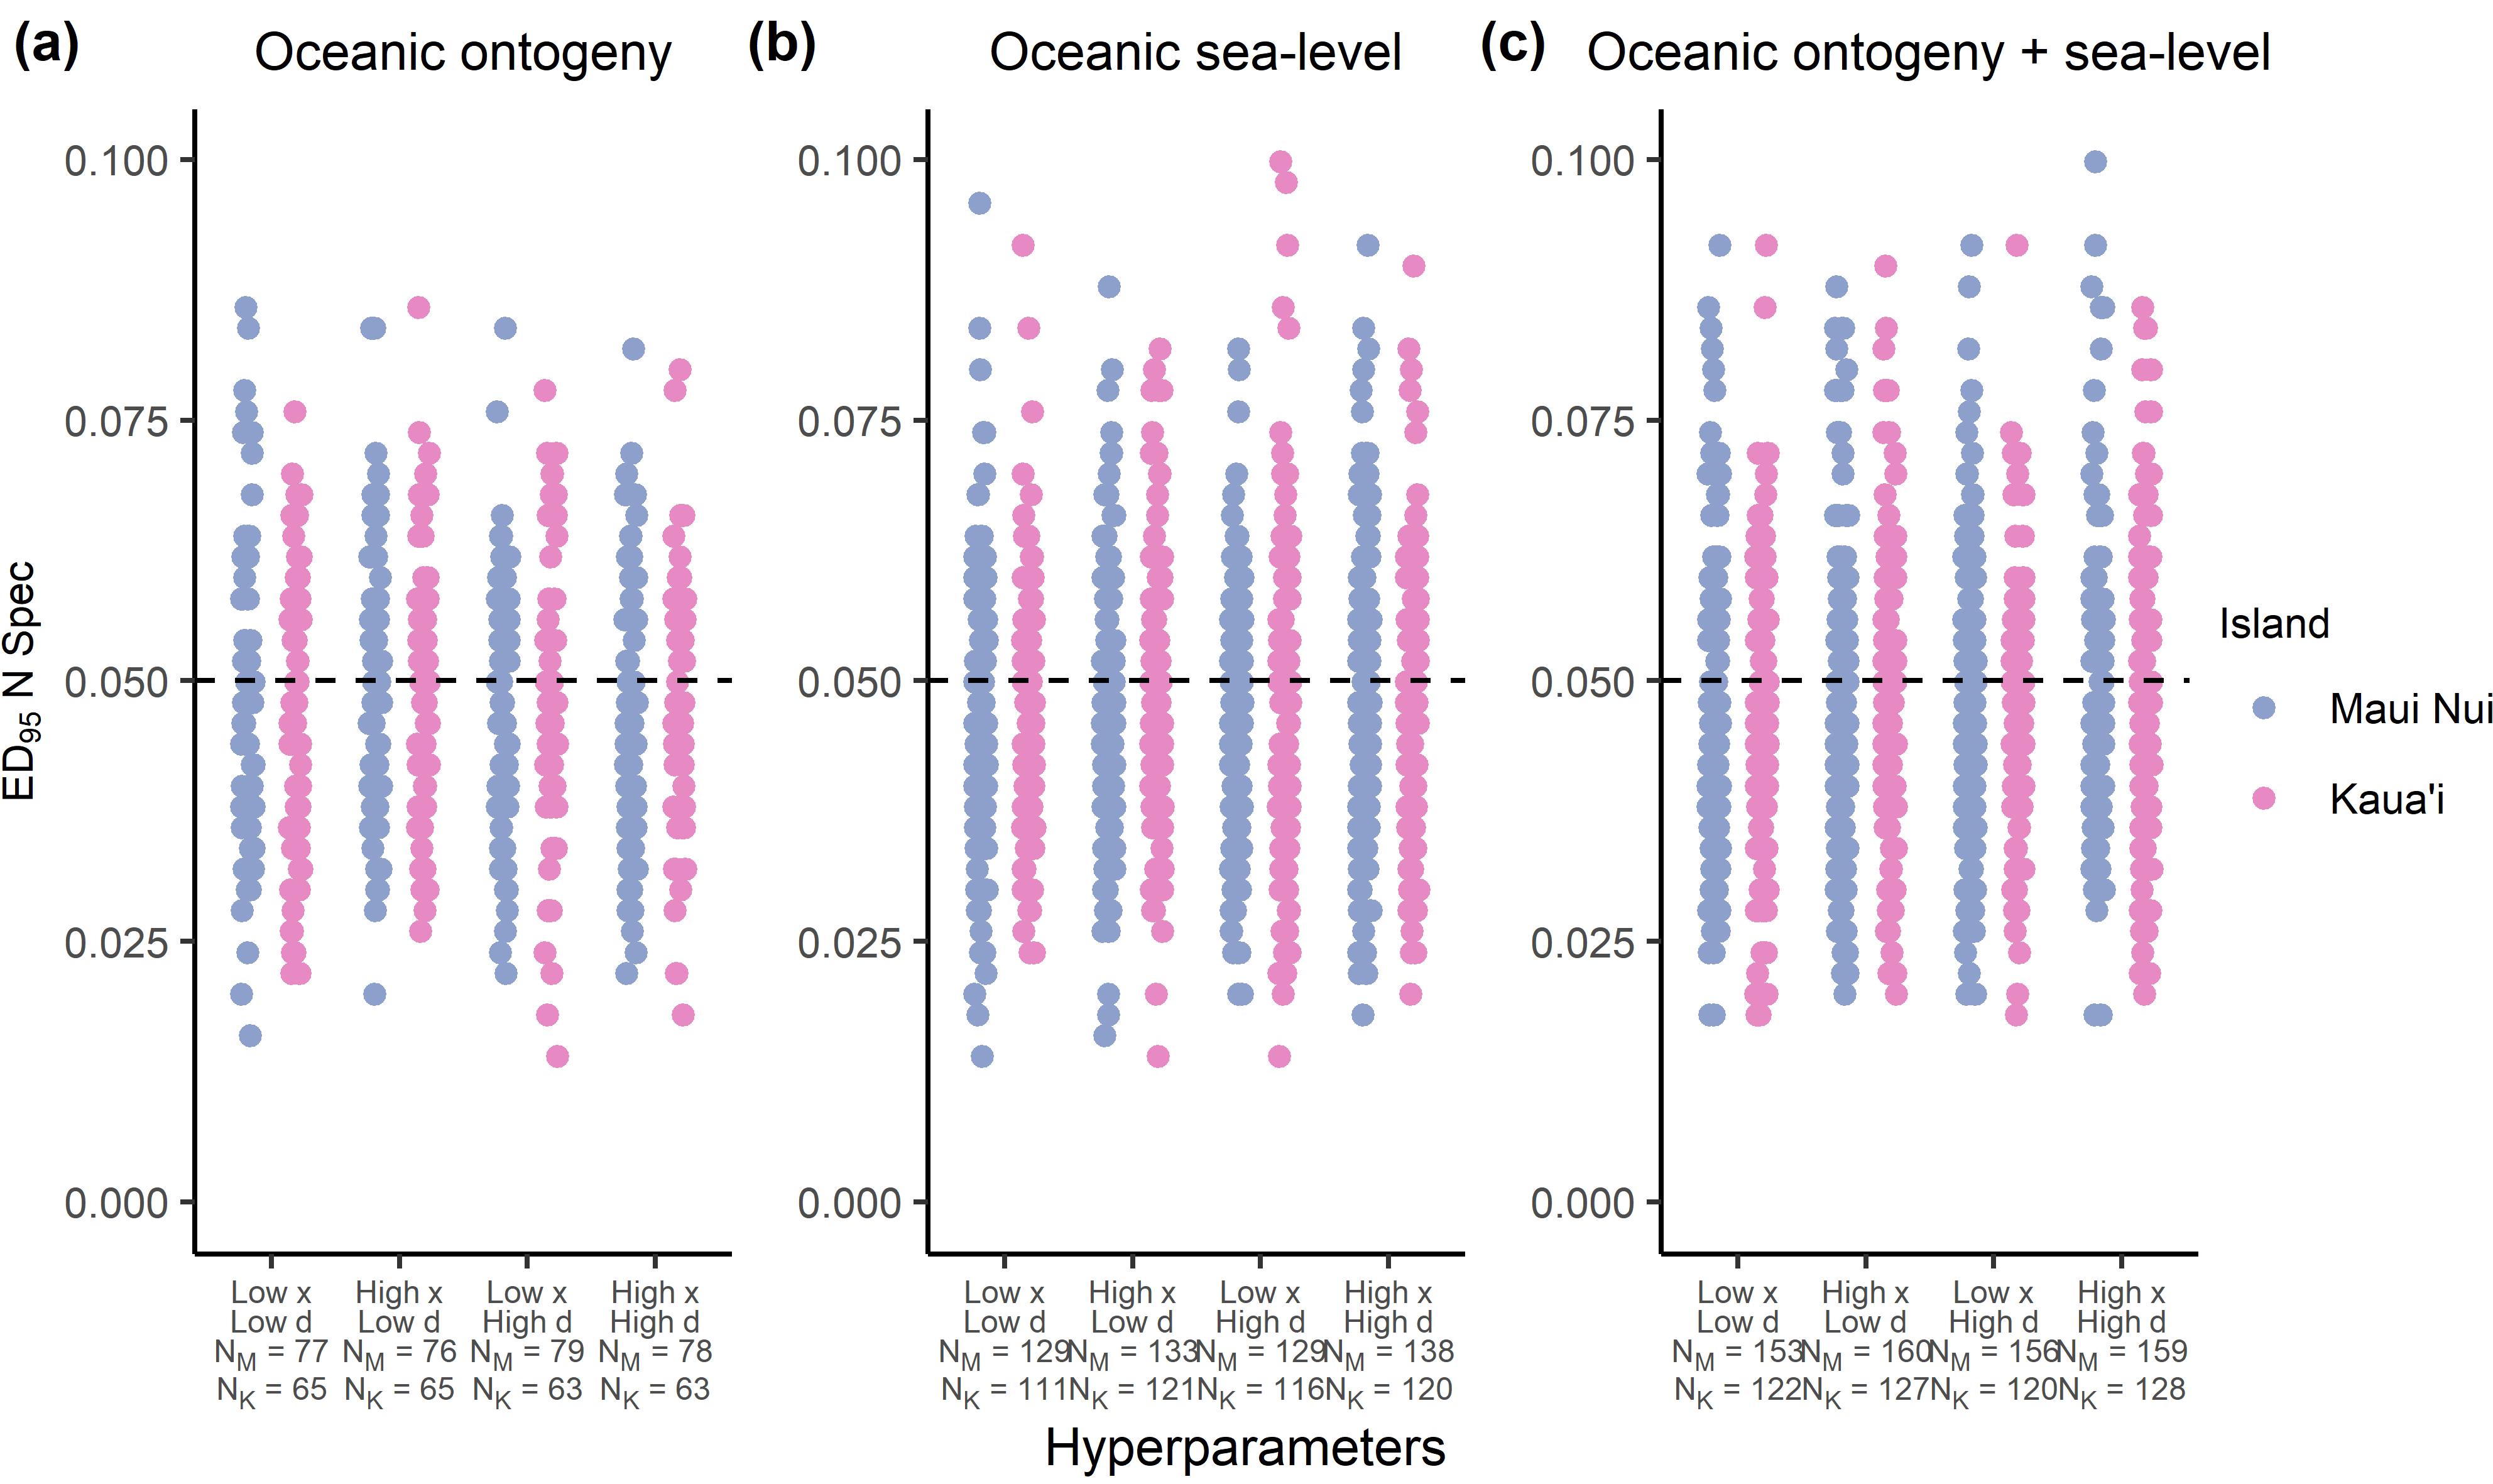
\includegraphics{Hyperparameters_num_spec.png}
    \caption{Strip charts showing the distributions of the ED\textsubscript{95} statistic for number of species at the present (at the end of the simulation) for each combination of hyperparameters (\textit{d} and \textit{x} controlling the effect of area on the rates of cladogenesis and extinction respectively). One point represents the ED\textsubscript{95} for a single parameter set with the specified hyperparameters on the \textit{x}-axis. All plots have a dashed line at 0.05 which is the null expectation of the ED\textsubscript{95}. (a) ED\textsubscript{95} statistic for number of species at the present for oceanic ontogeny. (b) ED\textsubscript{95} statistic for number of species at the present for oceanic sea-level. (c) ED\textsubscript{95} statistic for number of species at the present for oceanic ontogeny and sea-level. Sample size for young island (green) on each strip is given in the \textit{x}-axis label by N\textsubscript{Y}. Sample size for old island (orange) on each strip is given in the \textit{x}-axis label by N\textsubscript{O}.}
    \label{fig:Hyperparameters_num_spec}
\end{figure}

\begin{figure}
    \centering
    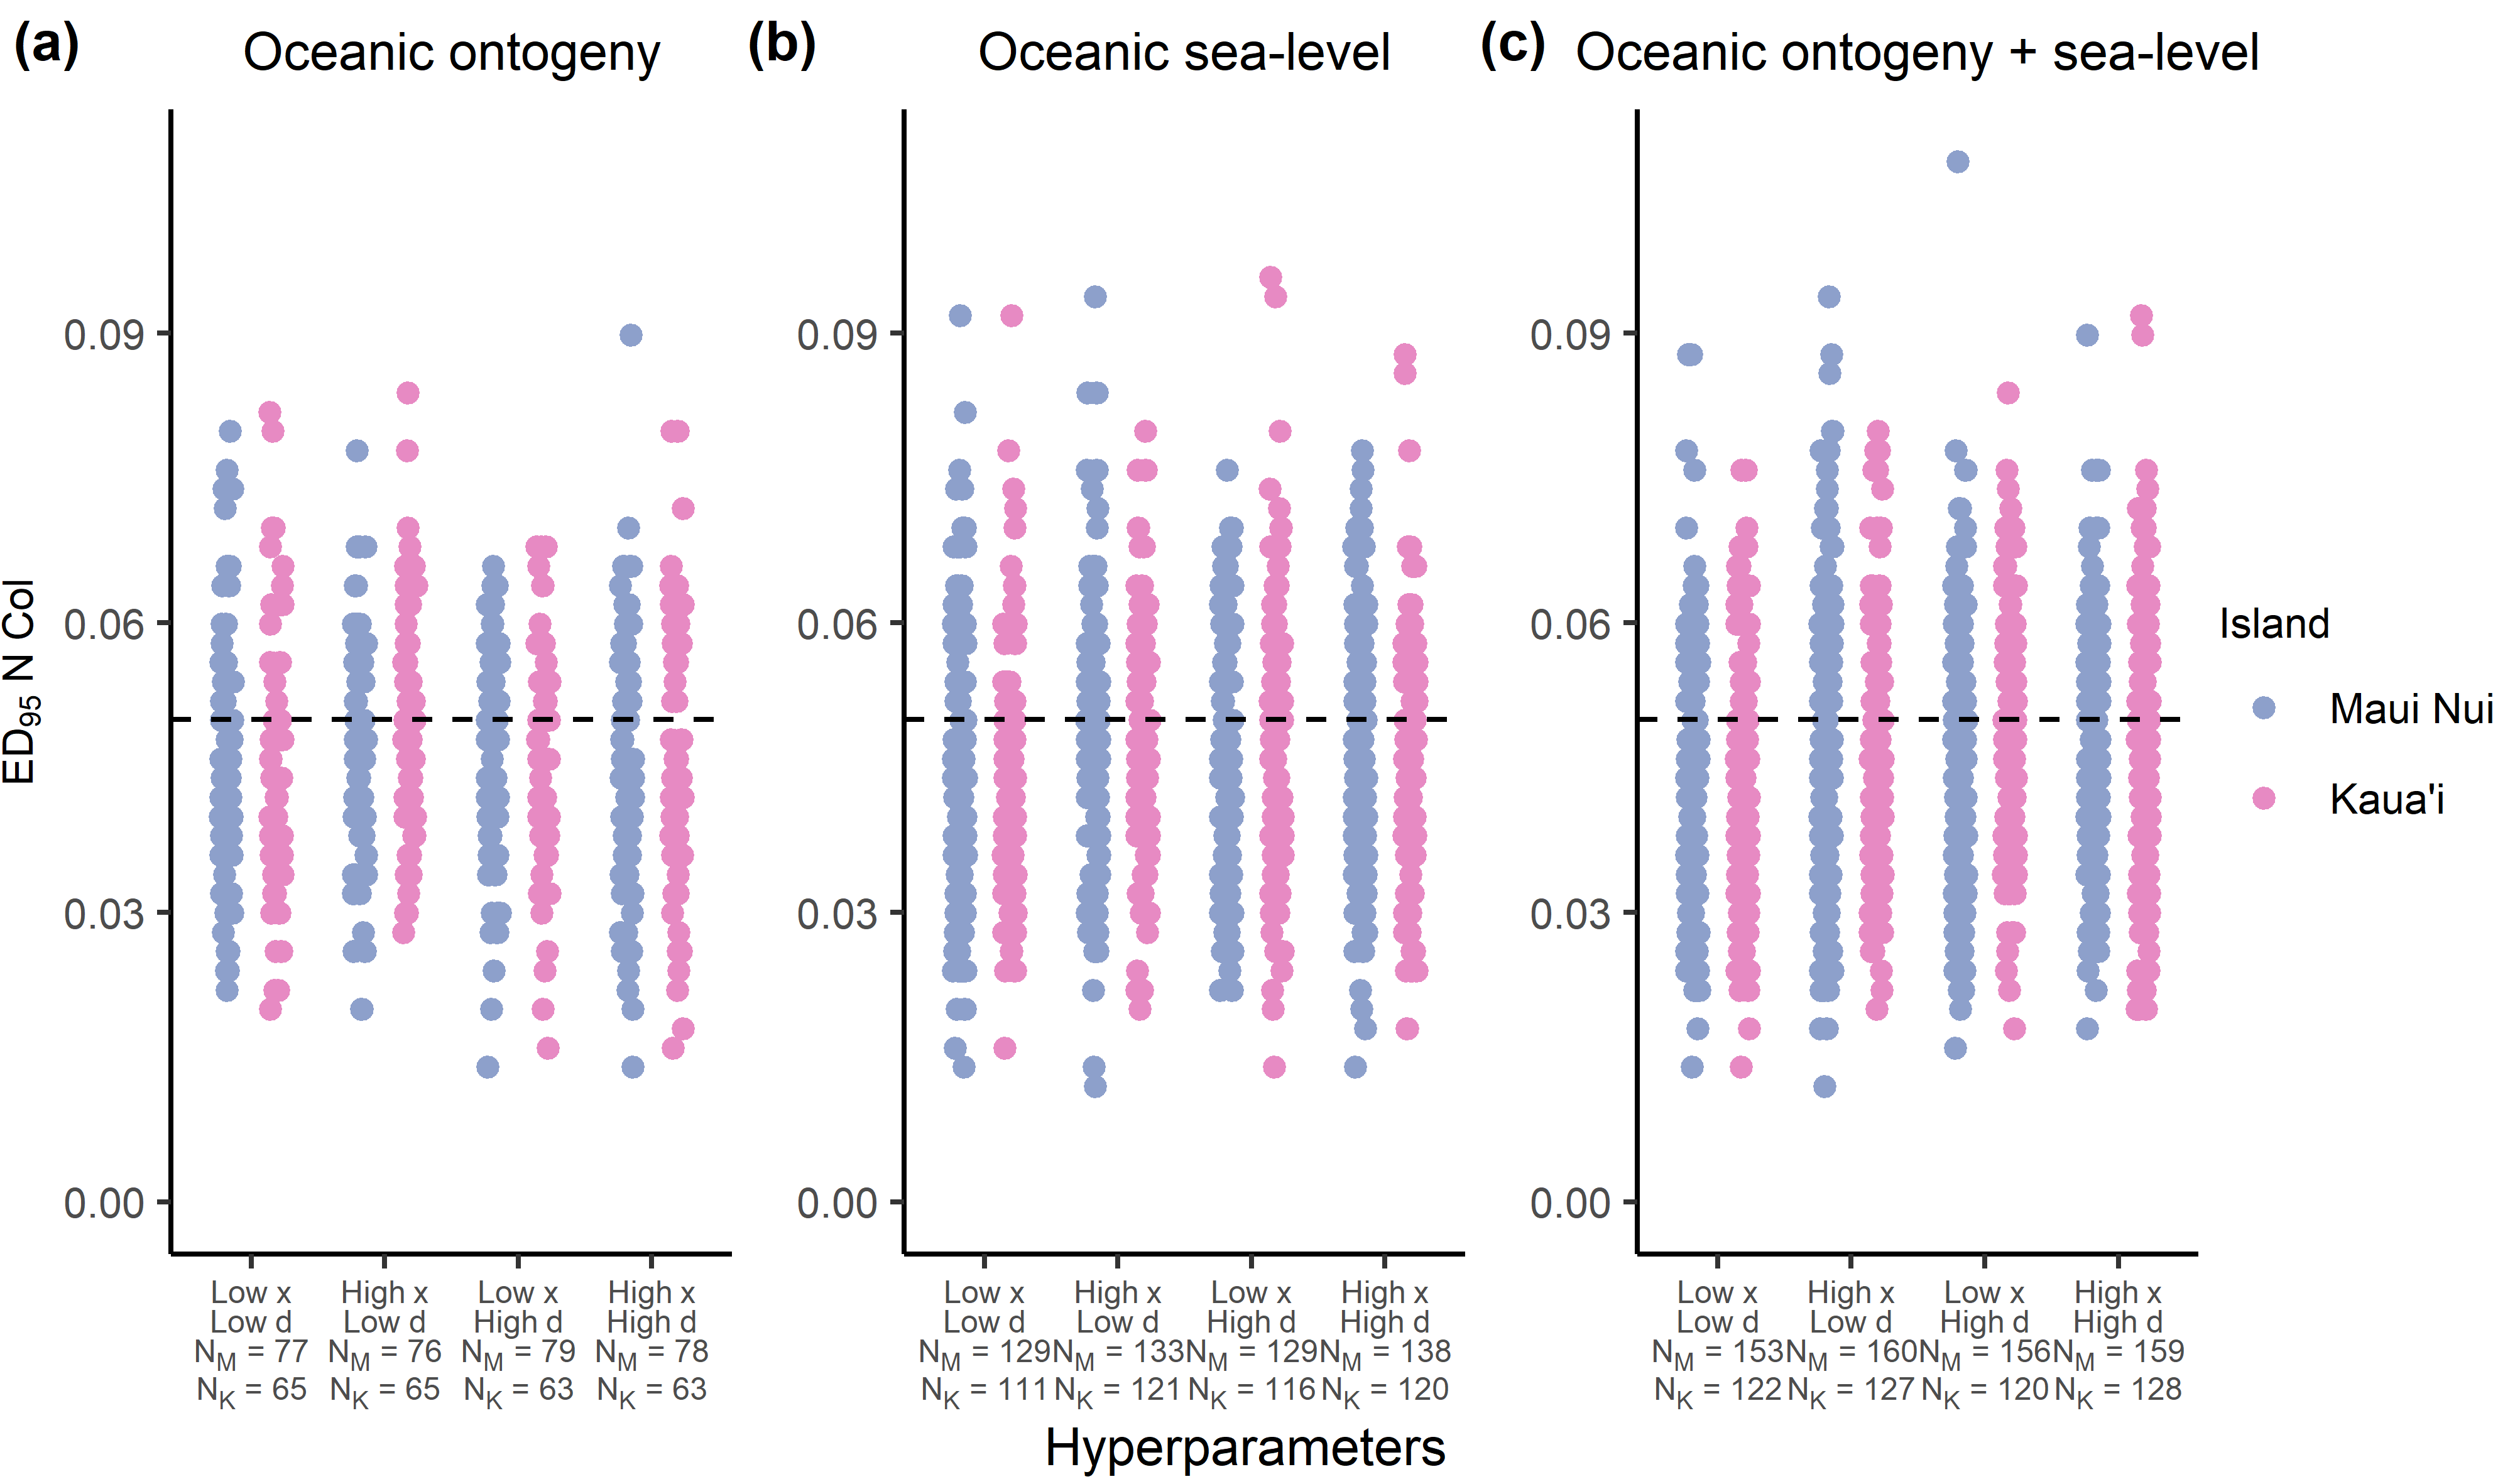
\includegraphics{Hyperparameters_num_col.png}
    \caption{Strip charts showing the distributions of the ED\textsubscript{95} statistic for number of colonists at the present (at the end of the simulation) for each combination of hyperparameters (\textit{d} and \textit{x} controlling the effect of area on the rates of cladogenesis and extinction respectively). One point represents the ED\textsubscript{95} for a single parameter set with the specified hyperparameters on the \textit{x}-axis. All plots have a dashed line at 0.05 which is the null expectation of the ED\textsubscript{95}. (a) ED\textsubscript{95} statistic for number of colonists at the present for oceanic ontogeny. (b) ED\textsubscript{95} statistic for number of colonists at the present for oceanic sea-level. (c) ED\textsubscript{95} statistic for number of colonists at the present for oceanic ontogeny and sea-level. Sample size for young island (green) on each strip is given in the \textit{x}-axis label by N\textsubscript{Y}. Sample size for old island (orange) on each strip is given in the \textit{x}-axis label by N\textsubscript{O}.}
    \label{fig:Hyperparameters_num_col}
\end{figure}

\begin{figure}
    \centering
    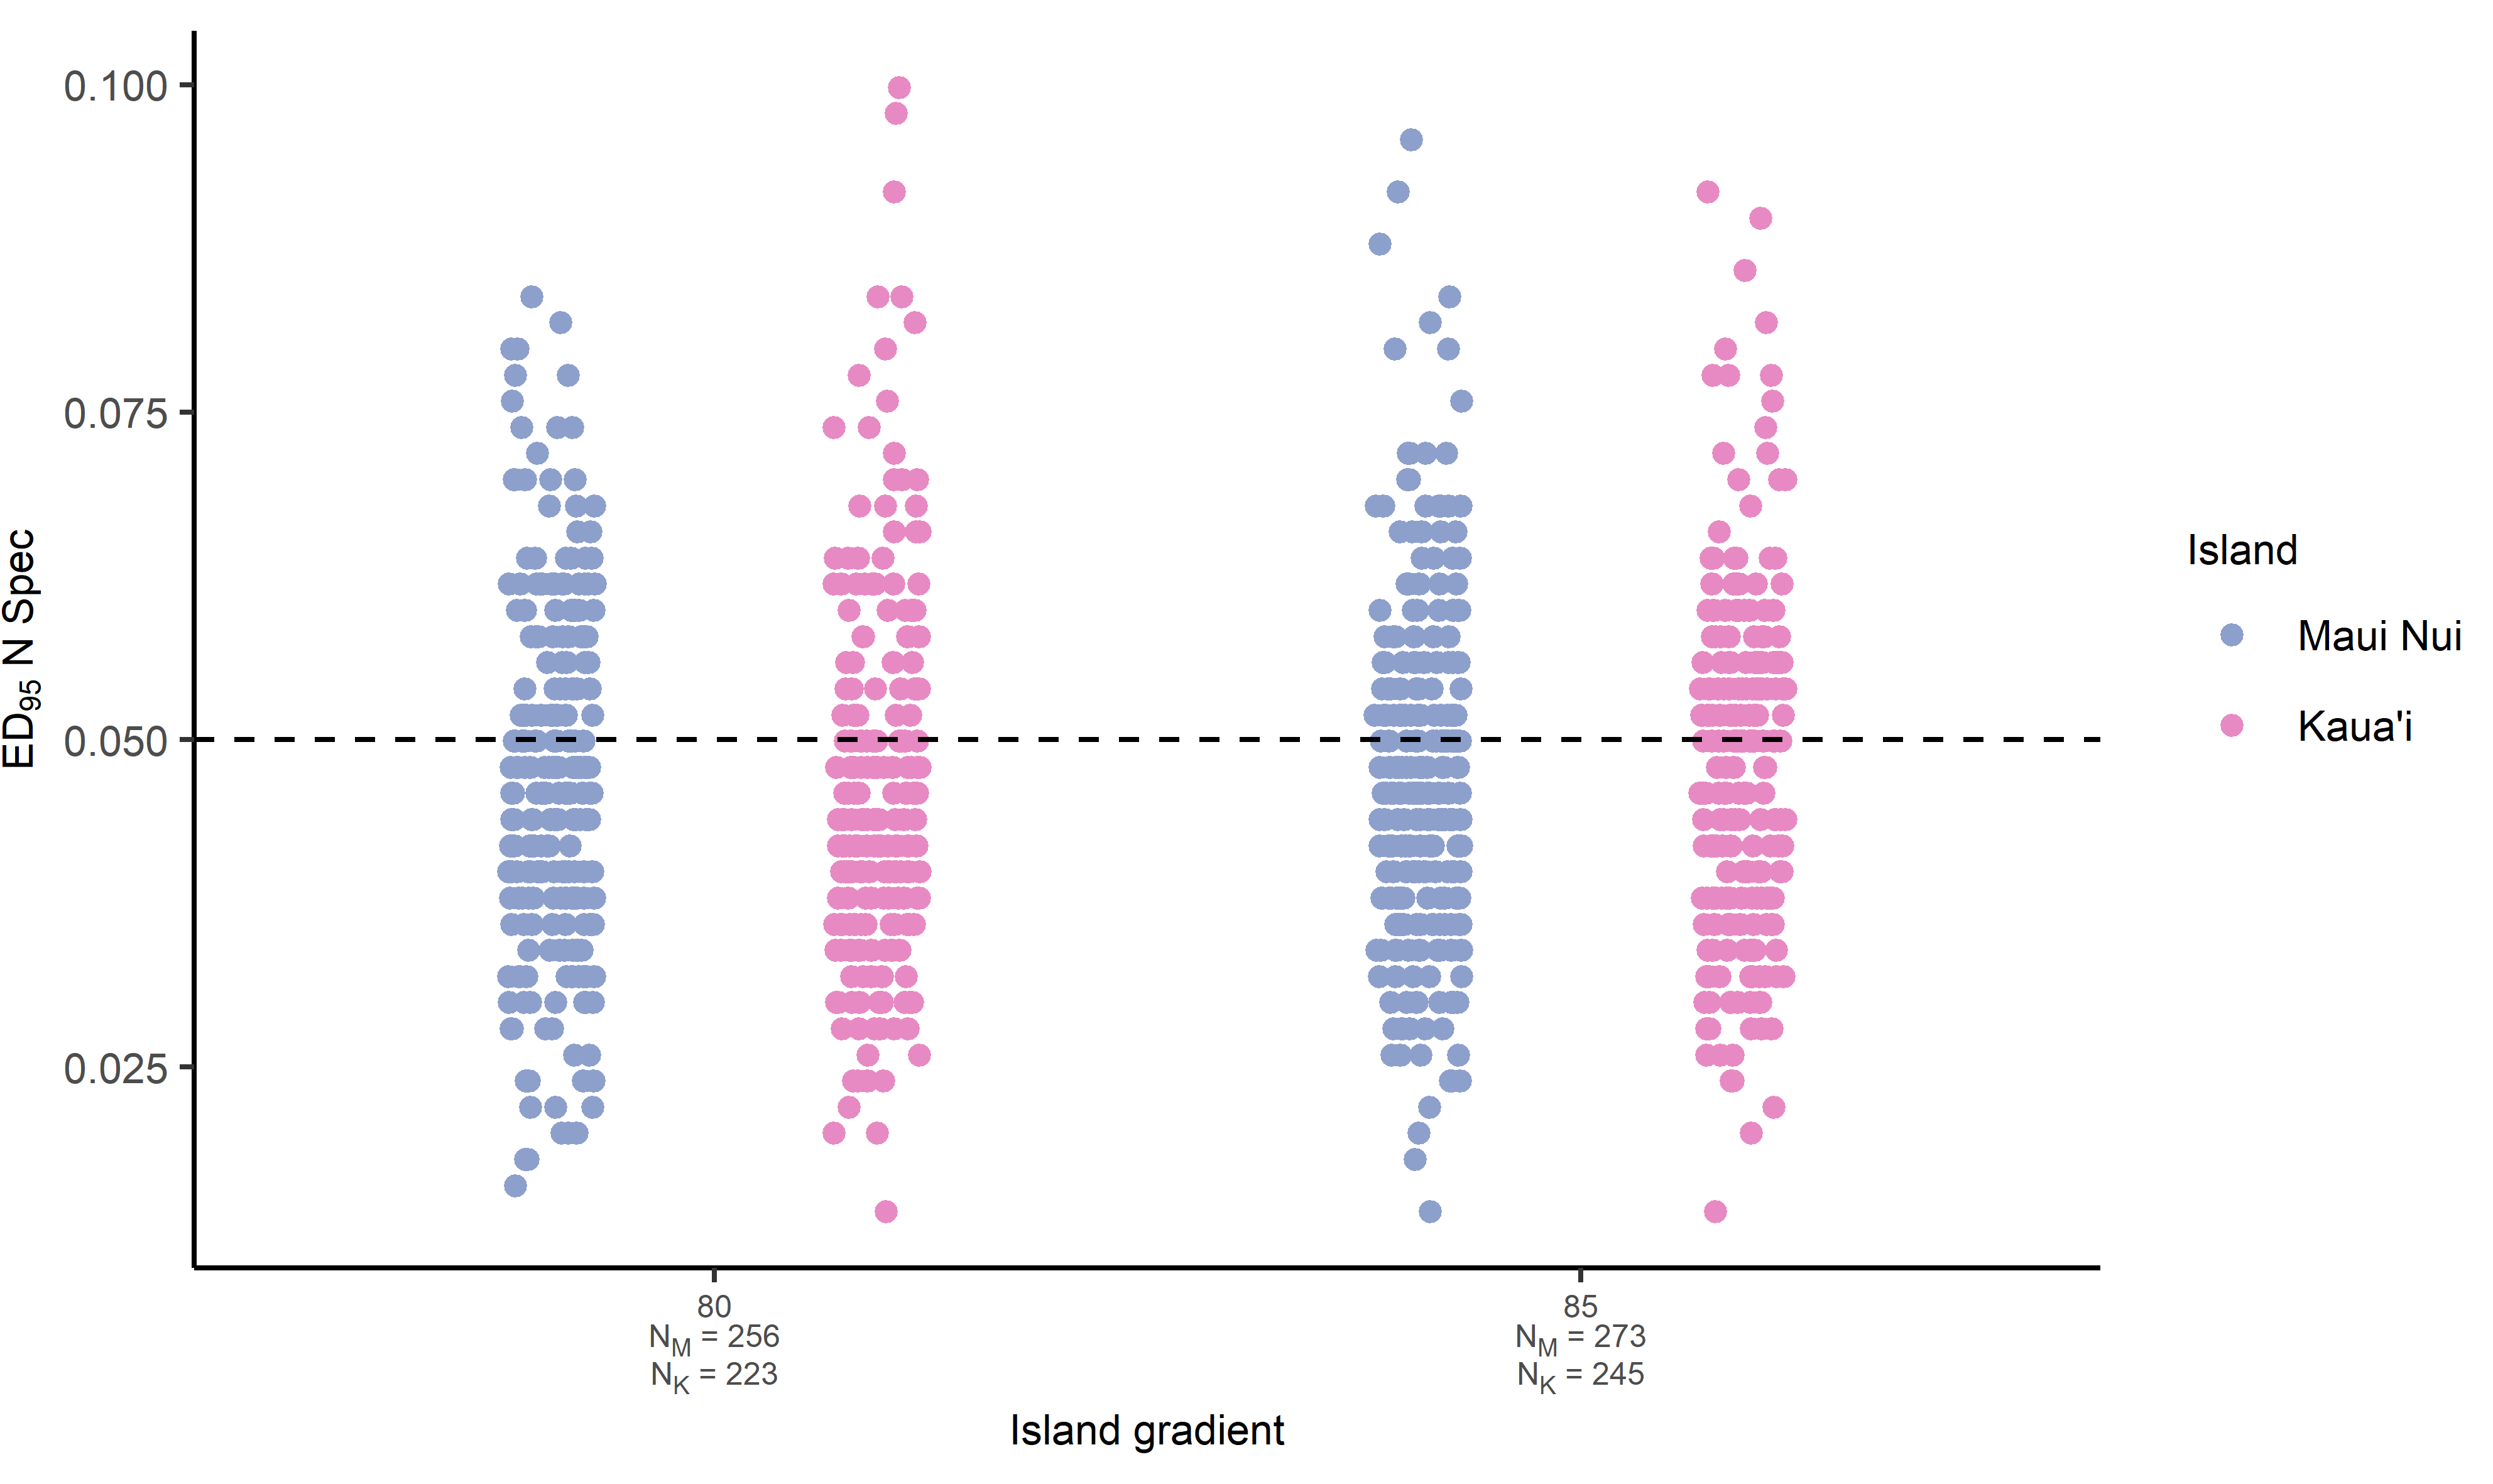
\includegraphics{Island_gradient_sea_level_num_spec.png}
    \caption{Strip charts showing the distributions of the ED\textsubscript{95} statistic for the number of species at the present (N Spec) for each combination of island gradients for oceanic sea-level. One point represents the ED\textsubscript{95} for a single parameter set with the specified island gradient on the \textit{x}-axis. All plots have a dashed line at 0.05 which is the null expectation of the ED\textsubscript{95}. ED\textsubscript{95} statistic for number of species at the present for oceanic sea-level. Sample size for young island (green) on each strip is given in the \textit{x}-axis label by N\textsubscript{Y}. Sample size for old island (orange) on each strip is given in the \textit{x}-axis label by N\textsubscript{O}.}
    \label{fig:Island_gradient_sea_level_num_spec}
\end{figure}

\begin{figure}
    \centering
    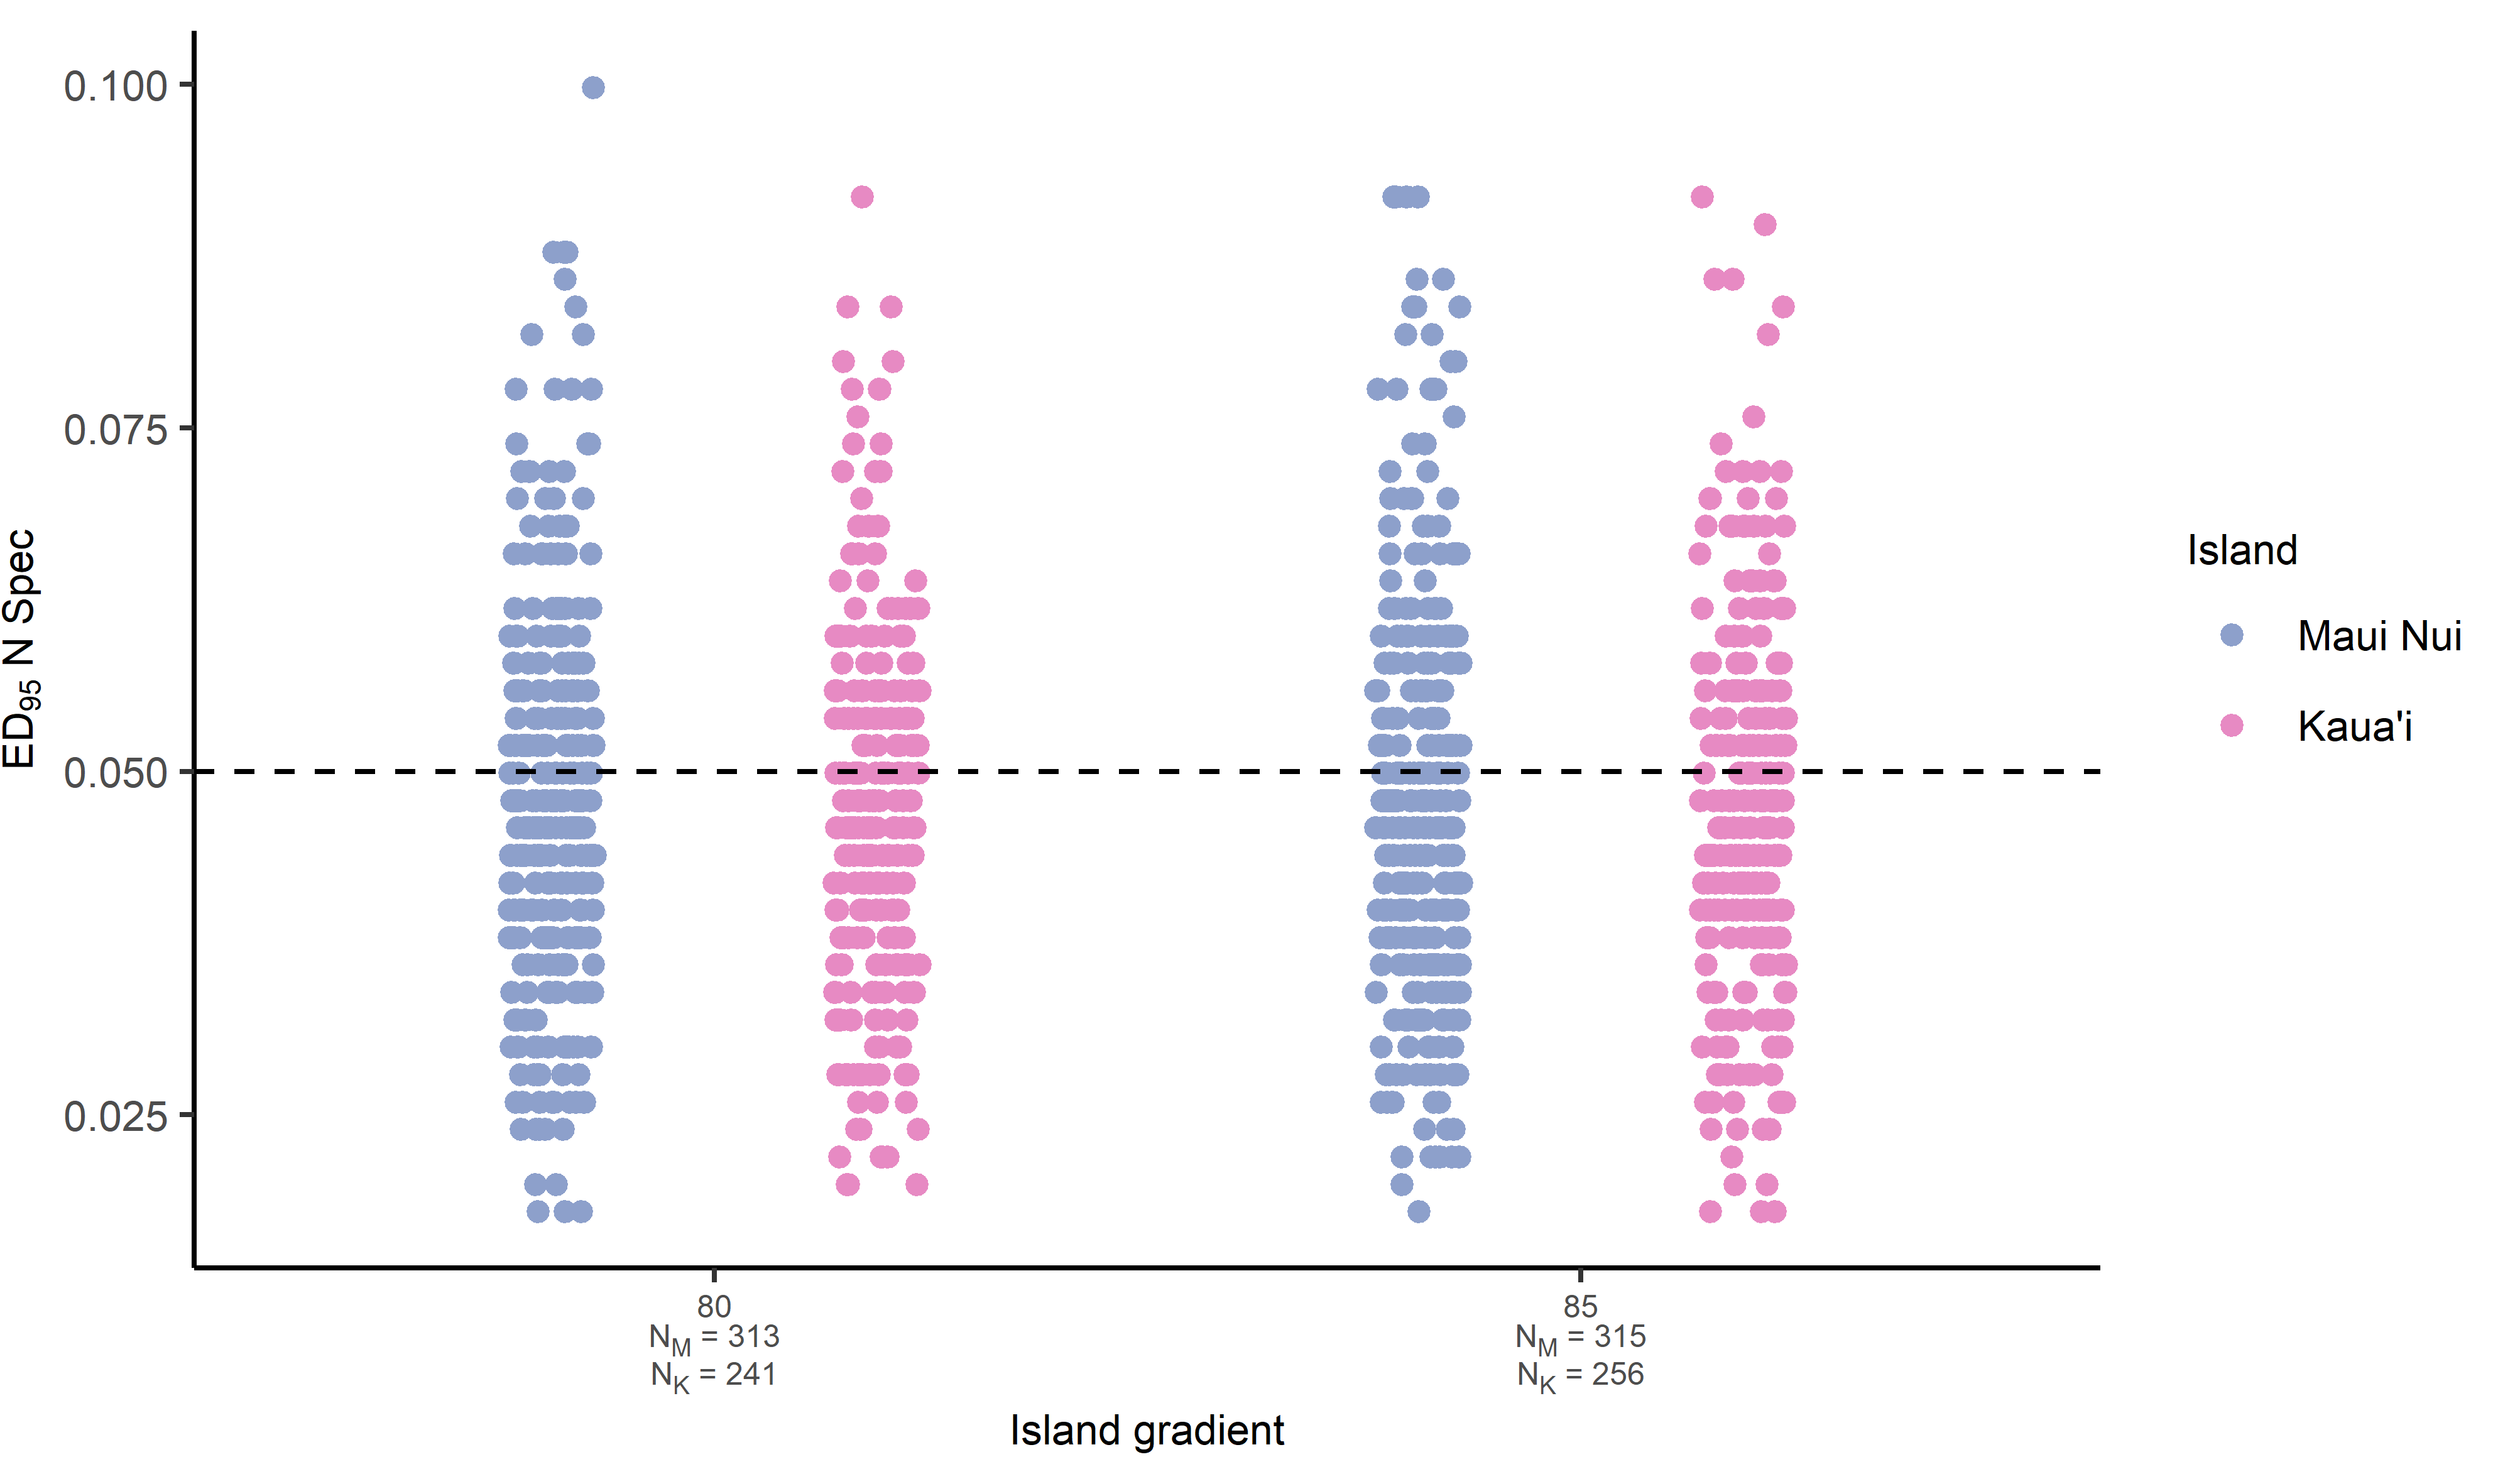
\includegraphics{Island_gradient_ontogeny_sea_level_num_spec.png}
    \caption{Strip charts showing the distributions of the ED\textsubscript{95} statistic for the number of species at the present (N Spec) for each combination of island gradients for oceanic ontogeny sea-level. One point represents the ED\textsubscript{95} for a single parameter set with the specified island gradient on the \textit{x}-axis. All plots have a dashed line at 0.05 which is the null expectation of the ED\textsubscript{95}. ED\textsubscript{95} statistic for number of species at the present for oceanic ontogeny sea-level. Sample size for young island (green) on each strip is given in the \textit{x}-axis label by N\textsubscript{Y}. Sample size for old island (orange) on each strip is given in the \textit{x}-axis label by N\textsubscript{O}.}
    \label{fig:Island_gradient_ontogeny_sea_level_num_spec}
\end{figure}

\begin{figure}
    \centering
    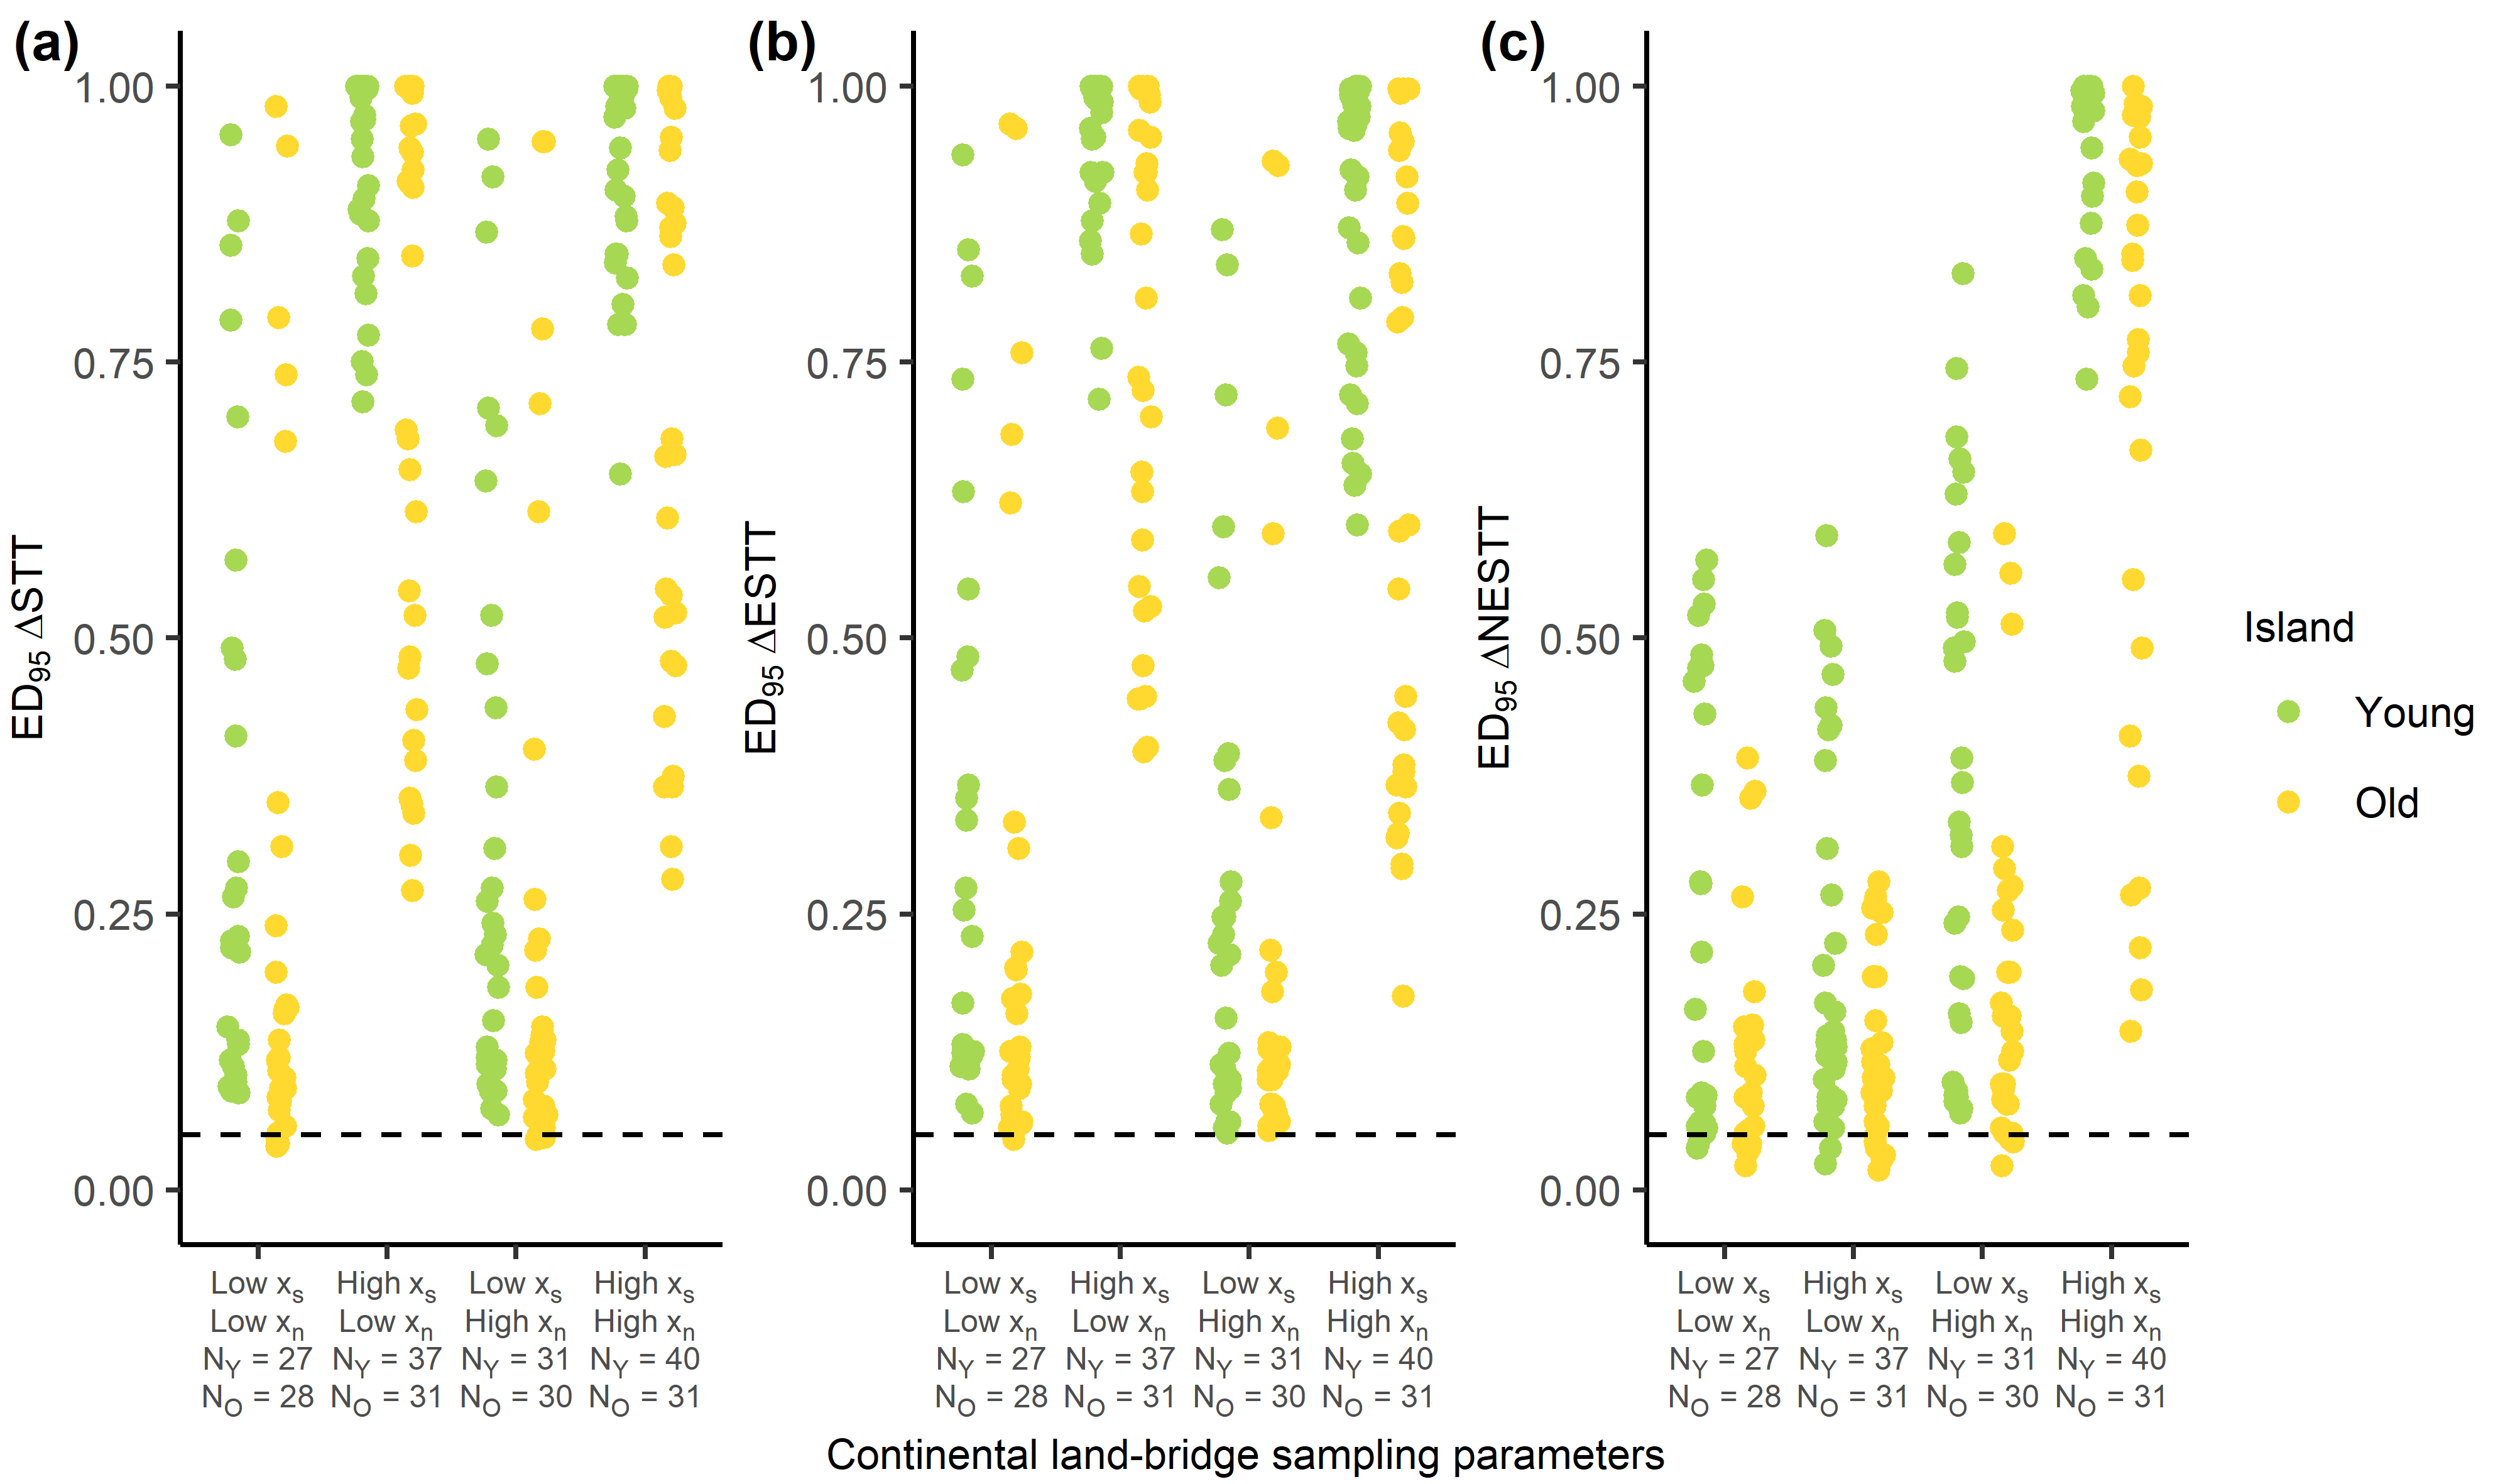
\includegraphics{continental_land_bridge_sample_facet.png}
    \caption{Strip charts showing the distributions of the ED\textsubscript{95} statistic for each combination of continental sampling parameters ($x_s$ and $x_n$ controlling the sampling probability of a species being initially present on the island and the sampling probability of species present initially on the island being non-endemic). One point represents the ED\textsubscript{95} for a single parameter set with the specified sampling parameters on the \textit{x}-axis. All plots have a dashed line at 0.05 which is the null expectation of the ED\textsubscript{95}. (a) $\Delta$STT ED\textsubscript{95} statistic, (b) $\Delta$ESTT ED\textsubscript{95} statistic, (c) $\Delta$NESTT ED\textsubscript{95} statistic for continental land-bridge. Sample size for young island (green) on each strip is given in the \textit{x}-axis label by N\textsubscript{Y}. Sample size for old island (orange) on each strip is given in the \textit{x}-axis label by N\textsubscript{O}.}
    \label{fig:continental_land_bridge_sample_facet}
\end{figure}

\begin{figure}
    \centering
    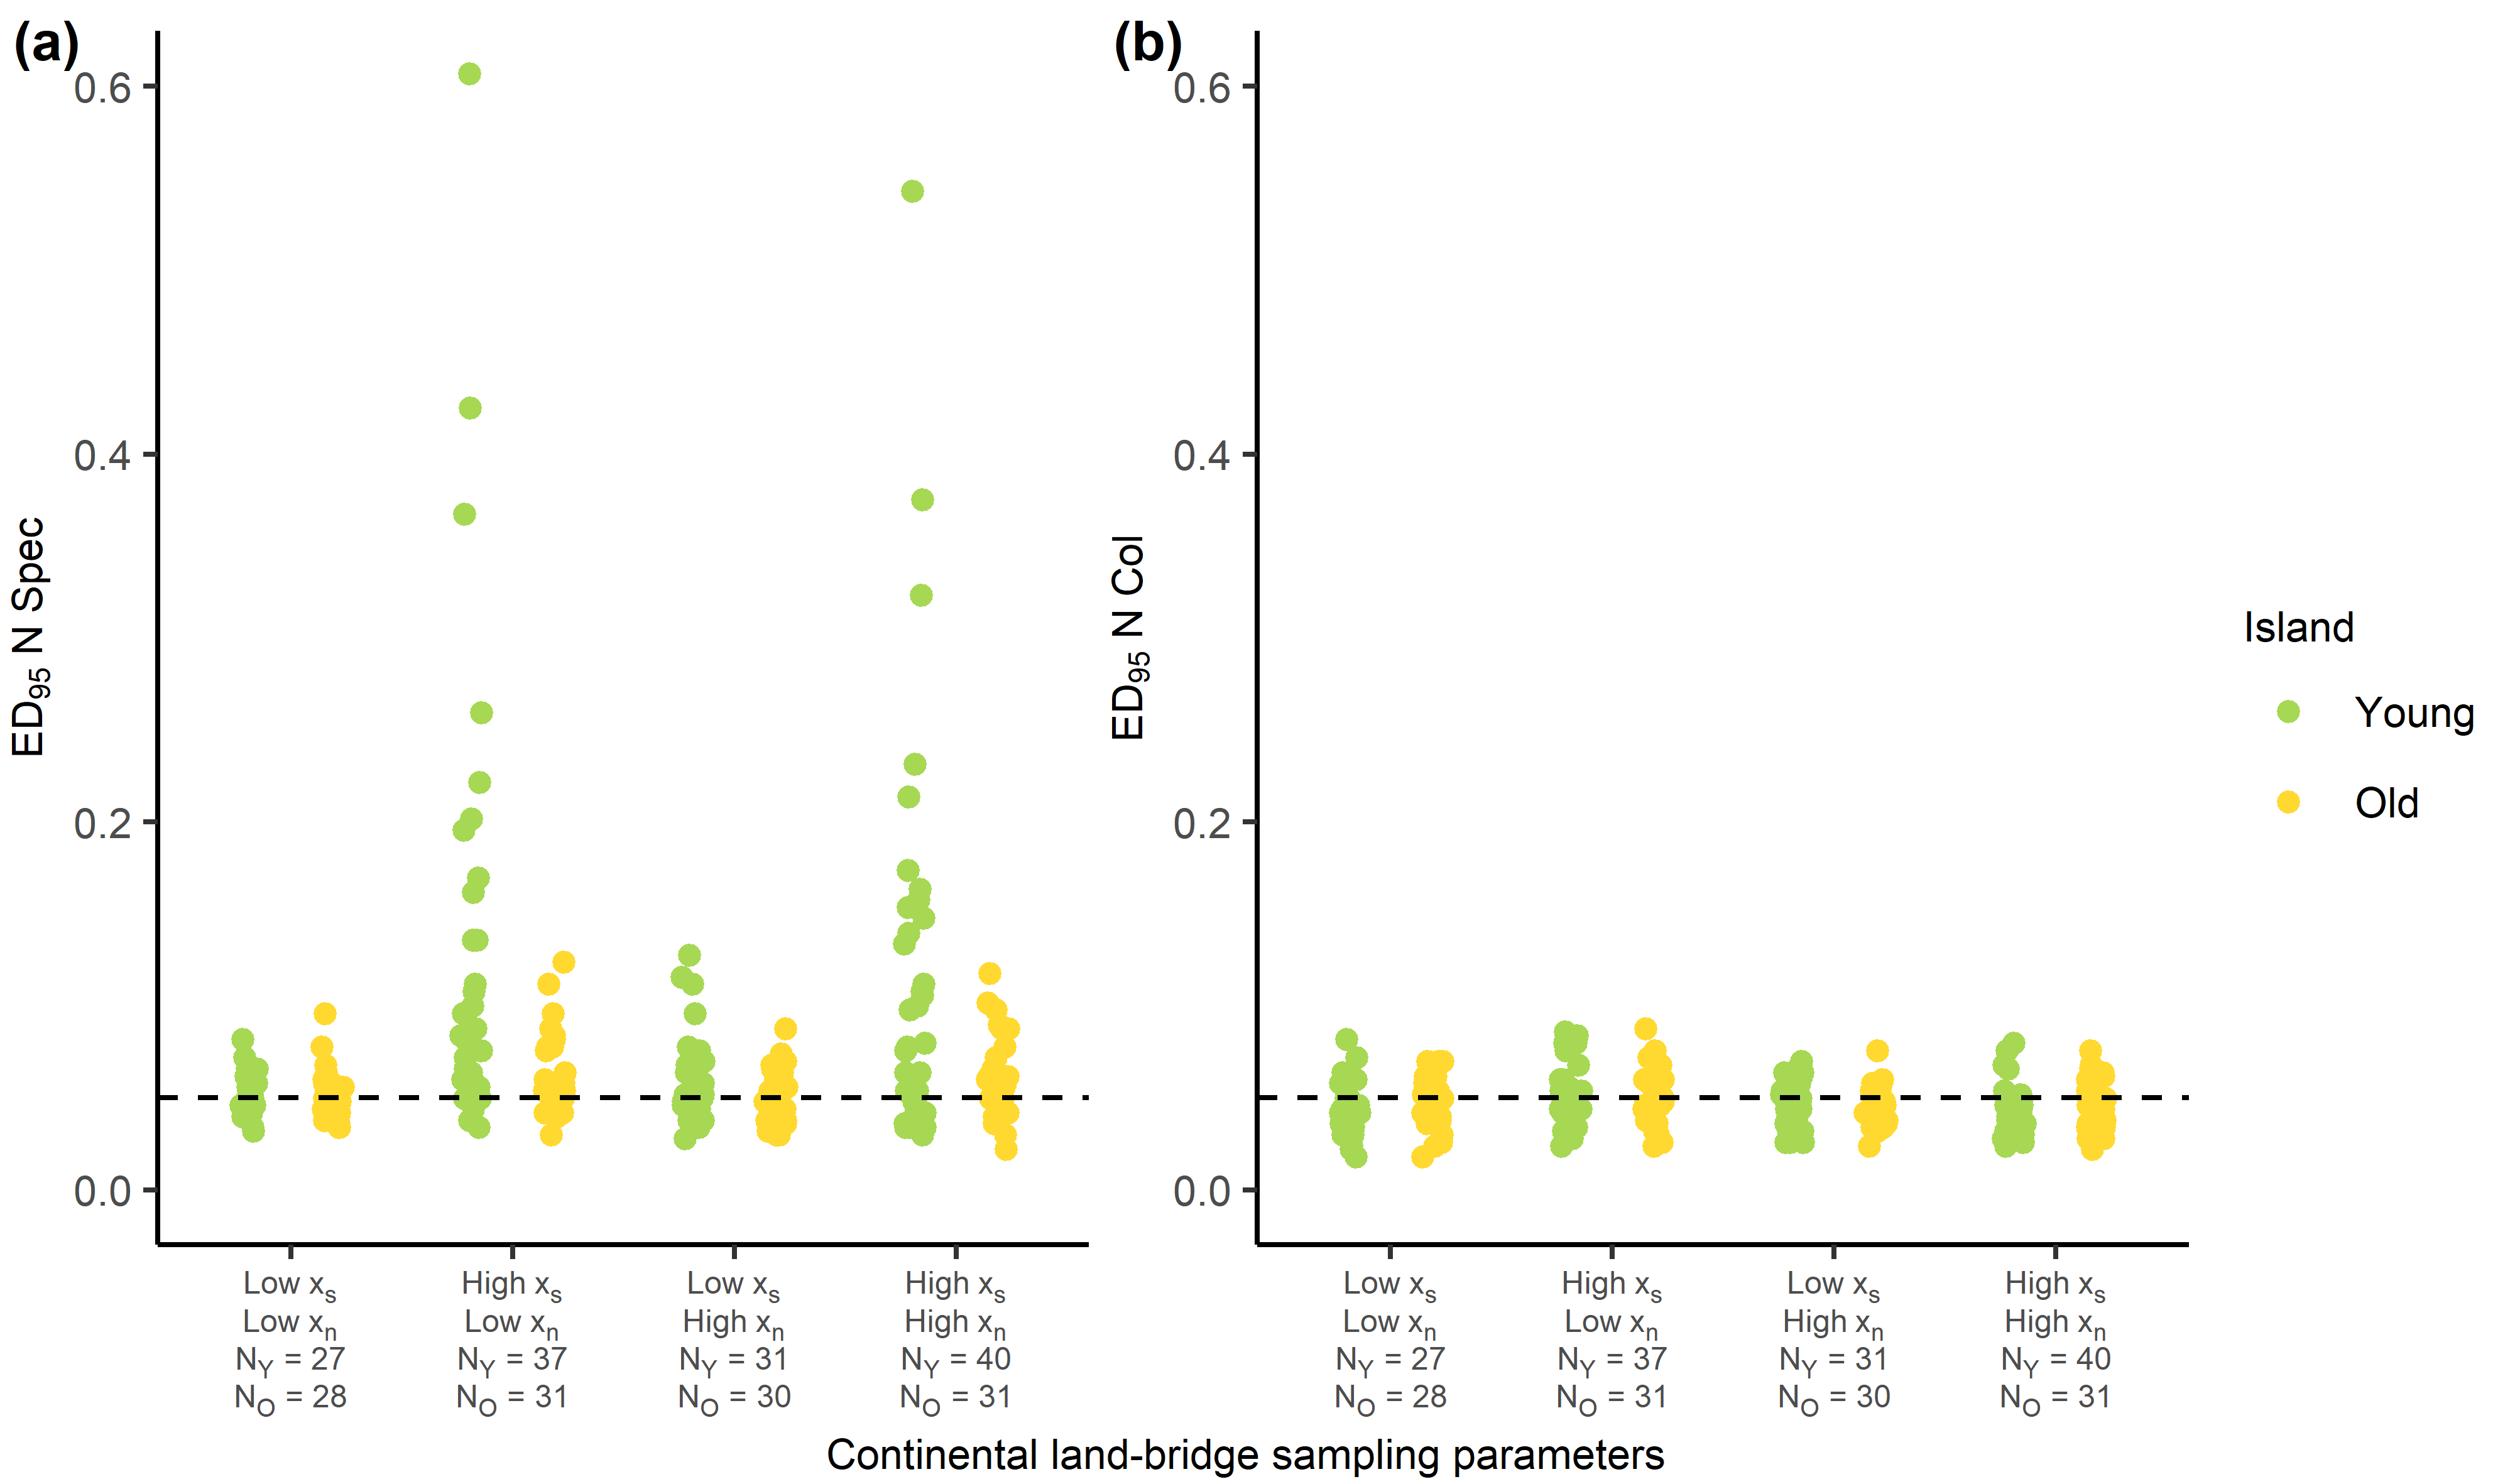
\includegraphics{continental_land_bridge_sample_spec_col_facet_.png}
    \caption{Strip charts showing the distributions of the ED\textsubscript{95} statistic for number of species (N Spec) (a) and colonists (N Col) (b) at the present for each combination of continental sampling parameters ($x_s$ and $x_n$ controlling the sampling probability of a species being initially present on the island and the sampling probability of species present initially on the island being non-endemic). One point represents the ED\textsubscript{95} for a single parameter set with the specified sampling parameters on the \textit{x}-axis. All plots have a dashed line at 0.05 which is the null expectation of the ED\textsubscript{95}. (a) $\Delta$STT ED\textsubscript{95} statistic, (b) $\Delta$ESTT ED\textsubscript{95} statistic, (c) $\Delta$NESTT ED\textsubscript{95} statistic for continental land-bridge. Sample size for young island (green) on each strip is given in the \textit{x}-axis label by N\textsubscript{Y}. Sample size for old island (orange) on each strip is given in the \textit{x}-axis label by N\textsubscript{O}.}
    \label{fig:continental_land_bridge_sample_spec_col_facet_}
\end{figure}

\begin{figure}
    \centering
    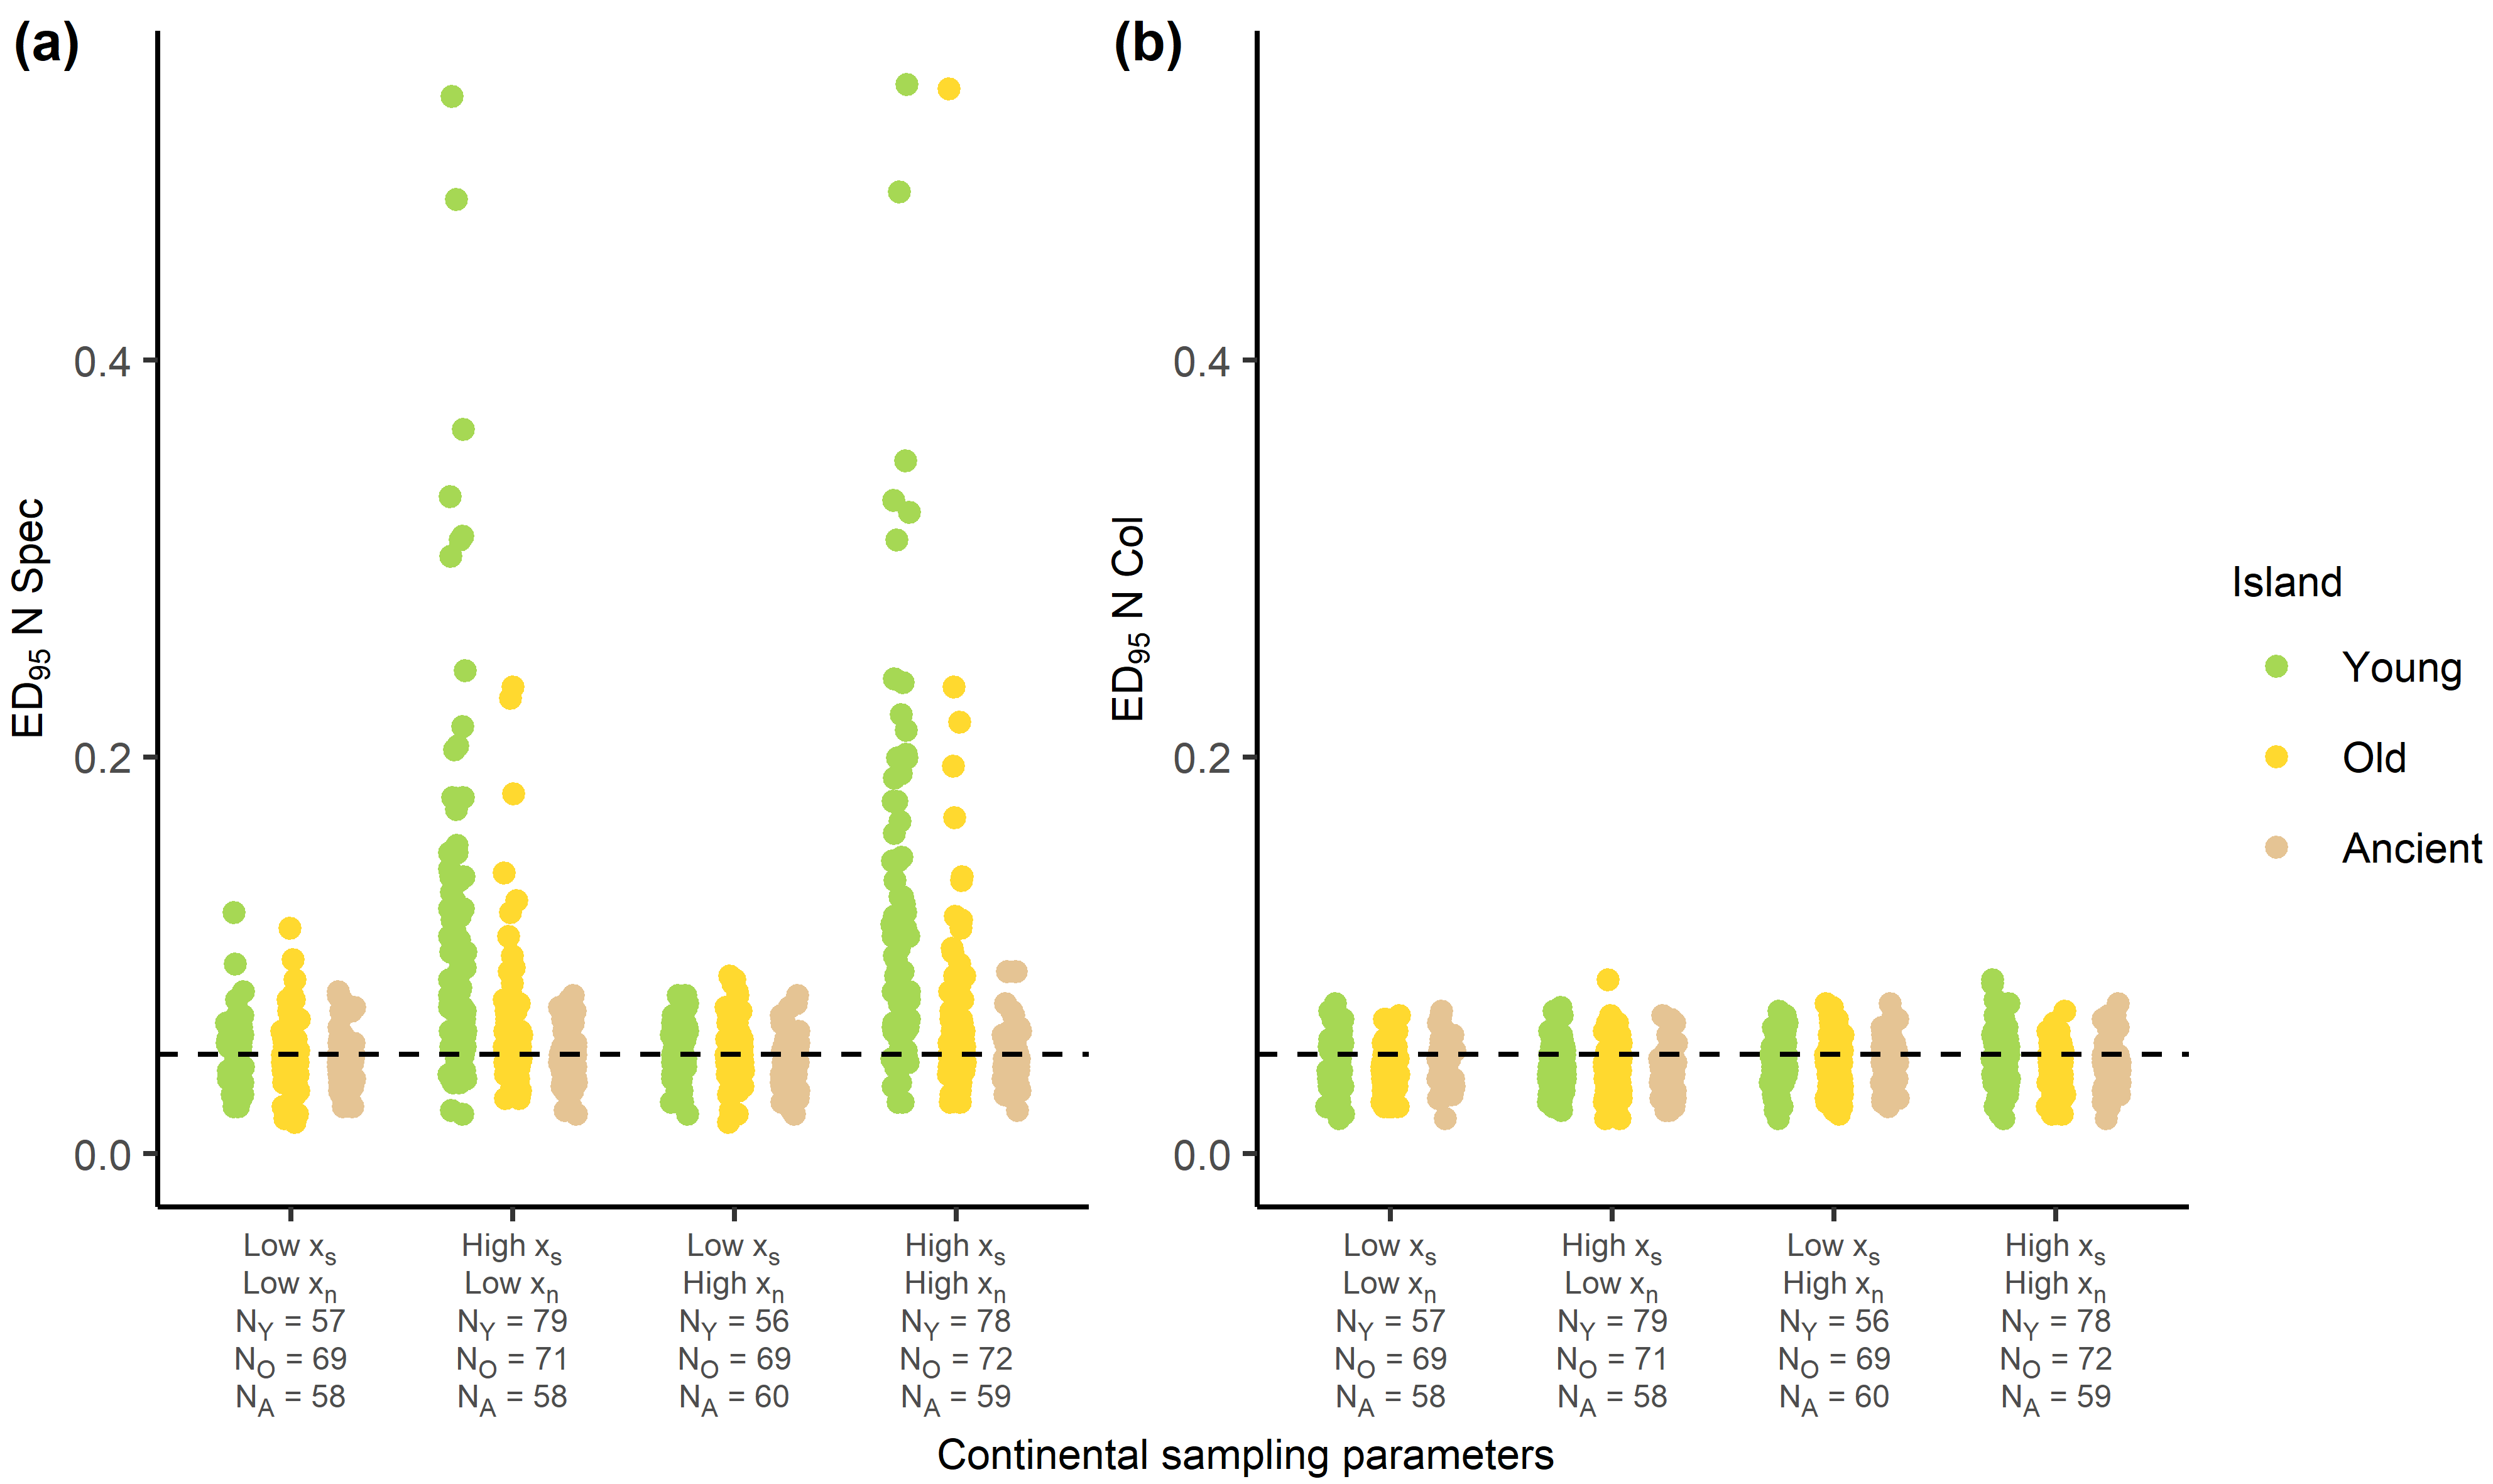
\includegraphics{continental_spec_col_facet_.png}
    \caption{Strip charts showing the distributions of the ED\textsubscript{95} statistic for number of species and colonists at the present for each combination of continental sampling parameters ($x_s$ and $x_n$ controlling the sampling probability of a species being initially present on the island and the sampling probability of species present initially on the island being non-endemic). One point represents the ED\textsubscript{95} for a single parameter set with the specified sampling parameters on the \textit{x}-axis. All plots have a dashed line at 0.05 which is the null expectation of the ED\textsubscript{95}. Sample size for young island (green) on each strip is given in the \textit{x}-axis label by N\textsubscript{Y}. Sample size for old island (orange) on each strip is given in the \textit{x}-axis label by N\textsubscript{O}. Sample size for the ancient island (blue) on each strip is given in the \textit{x}-axis label by N\textsubscript{A}.}
    \label{fig:continental_spec_col_facet_}
\end{figure}

\clearpage

\section*{Supplementary Tables}

\begin{table}[ht]
    \centering
    \caption{Parameter space for oceanic ontogeny young island. Parameter space consists of each combination of the model parameters.}
    \begin{tabular}{ c | c }
        \multicolumn{2}{c}{\textbf{Oceanic ontogeny young island}} \\
        \textbf{Model parameters} & \textbf{Parameter value} \\ 
        \hline
        \hline
        Time & 2.55 \\
        \hline
        Mainland species pool & 1000 \\
        \hline
        Cladogenesis & 0.02, 0.04 \\
        \hline
        Extinction & 0.975, 1.95 \\
        \hline
        Carrying capacity & 0.001, 0.01, $\infty$ \\
        \hline
        Colonisation & 0.03363, 0.06726 \\
        \hline
        Anagenesis & 0.0295, 0.059 \\
        \hline
        \textit{x} & 0.075, 0.15 \\
        \hline
        \textit{d} & 0.1108, 0.2216 \\
        \hline
        Max area & 13500 \\
        \hline
        Current area & 3155 \\
        \hline
        Peak time & 0.53 \\
        \hline
        Total island age & 2.864 \\
    \end{tabular}
    \label{tab:oceanic_ontogeny_young}
\end{table}

\begin{table}[ht]
    \centering
    \caption{Parameter space for oceanic ontogeny old island. Parameter space consists of each combination of the model parameters.}
    \begin{tabular}{ c | c }
        \multicolumn{2}{c}{\textbf{Oceanic ontogeny old island}} \\
        \textbf{Model parameters} & \textbf{Parameter value} \\ 
        \hline
        \hline
        Time & 6.15 \\
        \hline
        Mainland species pool & 1000 \\
        \hline
        Cladogenesis & 0.02, 0.04 \\
        \hline
        Extinction & 0.975, 1.95 \\
        \hline
        Carrying capacity & 0.001, 0.01, $\infty$ \\
        \hline
        Colonisation & 0.03363, 0.06726 \\
        \hline
        Anagenesis & 0.0295, 0.059 \\
        \hline
        \textit{x} & 0.075, 0.15 \\
        \hline
        \textit{d} & 0.1108, 0.2216 \\
        \hline
        Max area & 3787 \\
        \hline
        Current area & 1431 \\
        \hline
        Peak time & 0.27 \\
        \hline
        Total island age & 8.473 \\
    \end{tabular}
    \label{tab:oceanic_ontogeny_old}
\end{table}

\begin{table}[ht]
    \centering
    \caption{Parameter space for oceanic sea-level young island. Parameter space consists of each combination of the model parameters.}
    \begin{tabular}{ c | c }
        \multicolumn{2}{c}{\textbf{Oceanic sea-level young island}} \\
        \textbf{Model parameters} & \textbf{Parameter value} \\ 
        \hline
        \hline
        Time & 2.55 \\
        \hline
        Mainland species pool & 1000 \\
        \hline
        Cladogenesis & 0.02, 0.04 \\
        \hline
        Extinction & 0.975, 1.95 \\
        \hline
        Carrying capacity & 0.001, 0.01, $\infty$ \\
        \hline
        Colonisation & 0.03363, 0.06726 \\
        \hline
        Anagenesis & 0.0295, 0.059 \\
        \hline
        \textit{x} & 0.075, 0.15 \\
        \hline
        \textit{d} & 0.1108, 0.2216 \\
        \hline
        Current area & 3155 \\
        \hline
        Sea-level amplitude & 60 \\
        \hline
        Sea-level frequency & 25.5 \\
        \hline
        Island gradient angle & 80, 85 \\
    \end{tabular}
    \label{tab:oceanic_sea_level_young}
\end{table}

\begin{table}[ht]
    \centering
    \caption{Parameter space for oceanic sea-level old island. Parameter space consists of each combination of the model parameters.}
    \begin{tabular}{ c | c }
        \multicolumn{2}{c}{\textbf{Oceanic sea-level old island}} \\
        \textbf{Model parameters} & \textbf{Parameter value} \\ 
        \hline
        \hline
        Time & 6.15 \\
        \hline
        Mainland species pool & 1000 \\
        \hline
        Cladogenesis & 0.02, 0.04 \\
        \hline
        Extinction & 0.975, 1.95 \\
        \hline
        Carrying capacity & 0.001, 0.01, $\infty$ \\
        \hline
        Colonisation & 0.03363, 0.06726 \\
        \hline
        Anagenesis & 0.0295, 0.059 \\
        \hline
        \textit{x} & 0.075, 0.15 \\
        \hline
        \textit{d} & 0.1108, 0.2216 \\
        \hline
        Current area & 1431 \\
        \hline
        Sea-level amplitude & 60 \\
        \hline
        Sea-level frequency & 61.5 \\
        \hline
        Island gradient angle & 80, 85 \\
    \end{tabular}
    \label{tab:oceanic_sea_level_old}
\end{table}

\begin{table}[ht]
    \centering
    \caption{Parameter space for oceanic ontogeny sea-level young island. Parameter space consists of each combination of the model parameters.}
    \begin{tabular}{ c | c }
        \multicolumn{2}{c}{\textbf{Oceanic ontogeny sea-level young island}} \\
        \textbf{Model parameters} & \textbf{Parameter value} \\ 
        \hline
        \hline
        Time & 2.55 \\
        \hline
        Mainland species pool & 1000 \\
        \hline
        Cladogenesis & 0.02, 0.04 \\
        \hline
        Extinction & 0.975, 1.95 \\
        \hline
        Carrying capacity & 0.001, 0.01, $\infty$ \\
        \hline
        Colonisation & 0.03363, 0.06726 \\
        \hline
        Anagenesis & 0.0295, 0.059 \\
        \hline
        \textit{x} & 0.075, 0.15 \\
        \hline
        \textit{d} & 0.1108, 0.2216 \\
        \hline
        Max area & 13500 \\
        \hline
        Current area & 3155 \\
        \hline
        Peak time & 0.53 \\
        \hline
        Total island age & 2.864 \\
        \hline
        Sea-level amplitude & 60 \\
        \hline
        Sea-level frequency & 25.5 \\
        \hline
        Island gradient angle & 80, 85 \\
    \end{tabular}
    \label{tab:oceanic_ontogeny_sea_level_young}
\end{table}

\begin{table}[ht]
    \centering
    \caption{Parameter space for oceanic ontogeny sea-level old island. Parameter space consists of each combination of the model parameters.}
    \begin{tabular}{ c | c }
        \multicolumn{2}{c}{\textbf{Oceanic ontogeny sea-level old island}} \\
        \textbf{Model parameters} & \textbf{Parameter value} \\ 
        \hline
        \hline
        Time & 6.15 \\
        \hline
        Mainland species pool & 1000 \\
        \hline
        Cladogenesis & 0.02, 0.04 \\
        \hline
        Extinction & 0.975, 1.95 \\
        \hline
        Carrying capacity & 0.001, 0.01, $\infty$ \\
        \hline
        Colonisation & 0.03363, 0.06726 \\
        \hline
        Anagenesis & 0.0295, 0.059 \\
        \hline
        \textit{x} & 0.075, 0.15 \\
        \hline
        \textit{d} & 0.1108, 0.2216 \\
        \hline
        Max area & 3787 \\
        \hline
        Current area & 1431 \\
        \hline
        Peak time & 0.27 \\
        \hline
        Total island age & 8.473 \\
        \hline
        Sea-level amplitude & 60 \\
        \hline
        Sea-level frequency & 61.5 \\
        \hline
        Island gradient angle & 80, 85 \\
    \end{tabular}
    \label{tab:oceanic_ontogeny_sea_level_old}
\end{table}

\begin{table}[ht]
    \centering
    \caption{Parameter space for continental young, old and ancient islands. Parameter space consists of each combination of the model parameters.}
    \begin{tabular}{ c | c }
        \multicolumn{2}{c}{\textbf{Continental young, old, and ancient islands}} \\
        \textbf{Model parameters} & \textbf{Parameter value} \\ 
        \hline
        \hline
        Time & 2.55, 6.15, 50.00 \\
        \hline
        Mainland species pool & 1000 \\
        \hline
        Cladogenesis & 0.5, 1.0 \\
        \hline
        Extinction & 0.5, 1.0 \\
        \hline
        Carrying capacity & 10, 40, $\infty$ \\
        \hline
        Colonisation & 0.01, 0.05 \\
        \hline
        Anagenesis & 1.0, 2.0 \\
        \hline
        $x_s$ & 0.01, 0.05 \\
        \hline
        $x_n$ & 0.1, 0.9 \\
    \end{tabular}
    \label{tab:continental}
\end{table}

\begin{table}[ht]
    \centering
    \caption{Parameter space for continental land-bridge young island. Parameter space consists of each combination of the model parameters. Colonisation rate 2 (i.e. when the land-bridge is present) is colonisation rate 1 ($\gamma_1$), multipled by a colonisation rate multiplier, which in our case is two and ten.}
    \begin{tabular}{ c | c }
        \multicolumn{2}{c}{\textbf{Continental land-bridge young island}} \\
        \textbf{Model parameters} & \textbf{Parameter value} \\ 
        \hline
        \hline
        Time & 2.55 \\
        \hline
        Mainland species pool & 1000 \\
        \hline
        Cladogenesis 1 & 0.5, 1.0 \\
        \hline
        Extinction 1 & 0.5, 1.0 \\
        \hline
        Carrying capacity 1 & 10, $\infty$ \\
        \hline
        Colonisation 1 & 0.01, 0.05 \\
        \hline
        Anagenesis 1 & 1.0 \\
        \hline
        $x_s$ & 0.01, 0.05 \\
        \hline
        $x_n$ & 0.1, 0.9 \\
        \hline
        Cladogenesis 2 & 0.25, 0.5 \\
        \hline
        Extinction 2 & 0.25, 0.5 \\
        \hline
        Carrying capacity 2 & 10, $\infty$ \\
        \hline
        Colonisation 2 & $\gamma_1$ * 2, $\gamma_1$ * 10 \\ 
        \hline 
        Anagenesis 2 & 0 \\
        \hline
        Shift times & 1.225, 1.325 \\
    \end{tabular}
    \label{tab:continental_lb_young}
\end{table}

\begin{table}[ht]
    \centering
    \caption{Parameter space for continental land-bridge old island. Parameter space consists of each combination of the model parameters. Colonisation rate 2 (i.e. when the land-bridge is present) is colonisation rate 1 ($\gamma_1$), multipled by a colonisation rate multiplier, which in our case is two and ten.}
    \begin{tabular}{ c | c }
        \multicolumn{2}{c}{\textbf{Continental land-bridge old island}} \\
        \textbf{Model parameters} & \textbf{Parameter value} \\ 
        \hline
        \hline
        Time & 6.15 \\
        \hline
        Mainland species pool & 1000 \\
        \hline
        Cladogenesis 1 & 0.5, 1.0 \\
        \hline
        Extinction 1 & 0.5, 1.0 \\
        \hline
        Carrying capacity 1 & 10, $\infty$ \\
        \hline
        Colonisation 1 & 0.01, 0.05 \\
        \hline
        Anagenesis 1 & 1.0 \\
        \hline
        $x_s$ & 0.01, 0.05 \\
        \hline
        $x_n$ & 0.1, 0.9 \\
        \hline
        Cladogenesis 2 & 0.25, 0.5 \\
        \hline
        Extinction 2 & 0.25, 0.5 \\
        \hline
        Carrying capacity 2 & 10, $\infty$ \\
        \hline
        Colonisation 2 & $\gamma_1$ * 2, $\gamma_1$ * 10 \\ 
        \hline 
        Anagenesis 2 & 0 \\
        \hline
        Shift times & 3.025, 3.125 \\
    \end{tabular}
    \label{tab:continental_lb_old}
\end{table}
